%%%%%%%%%%%%%%%%%%%%%%%%%%%%% Thesis.tex %%%%%%%%%%%%%%%%%%%%%%%%%%%%%%%
%                                                                      %
%  ---------- Master of Science Dissertation template ----------       %
%                                                                      %
%  Template for the Master Thesis according to the regulations         %
%  published by the Academic Board (Direcção Académica) at IST.        %
%                                                                      %
%  For up-to-date guide, please refer to the official website          %
%  http://academica.tecnico.ulisboa.pt/alunos/dissertacao-de-mestrado/ %
%                                                                      %
%       Andre C. Marta                                                 %
%       Area Cientifica de Mecanica Aplicada e Aeroespacial            %
%       Departamento de Engenharia Mecanica                            %
%       Instituto Superior Tecnico                                     %
%       Av. Rovisco Pais                                               %
%       1049-001 Lisboa                                                %
%       Portugal                                                       %
%       Tel: +351 21 841 9469                                          %
%                        3469 (extension)                              %
%       Email: andre.marta@tecnico.ulisboa.pt                          %
%                                                                      %
%  Created:       Jan 20, 2011                                         %
%  Last Modified: Feb 19, 2018                                         %
%                                                                      %
%%%%%%%%%%%%%%%%%%%%%%%%%%%%%%%%%%%%%%%%%%%%%%%%%%%%%%%%%%%%%%%%%%%%%%%%
%  Revision history                                                    %
%  v1 - 2011/01/24 - original template                                 %
%  v2 - 2012/10/30 - new IST image and glossary support                %
%  v3 - 2013/12/10 - update according to 2012/13 official guide        %
%  v4 - 2014/02/28 - new default for bibliography style                %
%  v5 - 2014/05/07 - update according to 2013/14 official guide        %
%  v6 - 2015/07/02 - cover page format fixed,                          %
%                    contents page numbering fixed,                    %
%                    better language support,                          %
%                    enhanced examples of tables,                      %
%                    new option for appendix page numbering format,    %
%                    custom bibliography style                         %
%  v7 - 2018/02/19 - multiple citations compressed                     %
%%%%%%%%%%%%%%%%%%%%%%%%%%%%%%%%%%%%%%%%%%%%%%%%%%%%%%%%%%%%%%%%%%%%%%%%
%                                                                      %
% To generate the PDF file, type "make" at the terminal prompt.        %
%                                                                      %
% The IST template LaTeX package was created by the author             %
% and it can be downloaded from:                                       %
% https://fenix.ist.utl.pt/homepage/ist31052/                          %
%                                                                      %
% The external packages can be downloaded from                         %
% the Comprehensive TeX Archive Network at http://www.ctan.org/        %
%                                                                      %
% List of LaTex symbols:                                               %
% http://www.ctan.org/tex-archive/info/symbols/comprehensive/          %
%                                                                      %
% Help with LaTex can be found at                                      %
% http://www.giss.nasa.gov/tools/latex/ltx-2.html                      %
% http://en.wikibooks.org/wiki/LaTeX                                   %
%%%%%%%%%%%%%%%%%%%%%%%%%%%%%%%%%%%%%%%%%%%%%%%%%%%%%%%%%%%%%%%%%%%%%%%%

%%%%%%%%%%%%%%%%%%%%%%%%%%%%%%%%%%%%%%%%%%%%%%%%%%%%%%%%%%%%%%%%%%%%%%%%
%     Preamble                                                         %
%%%%%%%%%%%%%%%%%%%%%%%%%%%%%%%%%%%%%%%%%%%%%%%%%%%%%%%%%%%%%%%%%%%%%%%%

% ----------------------------------------------------------------------
%  Set the document class
% ----------------------------------------------------------------------
\documentclass[10pt,a4paper,twoside]{report}

% ----------------------------------------------------------------------
% Define external packages, language, margins, fonts and new commands
% ----------------------------------------------------------------------
\usepackage{listings}
\usepackage{color}
\usepackage[printonlyused]{acronym}
\usepackage[all]{nowidow}

\definecolor{dkgreen}{rgb}{0,0.6,0}
\definecolor{gray}{rgb}{0.5,0.5,0.5}
\definecolor{mauve}{rgb}{0.58,0,0.82}

\lstset{frame=tb,
	language=C,
	aboveskip=5mm,
	belowskip=5mm,
	showstringspaces=false,
	columns=flexible,
	basicstyle={\small\ttfamily},
	numbers=none,
	numberstyle=\tiny\color{gray},
	keywordstyle=\color{blue},
	commentstyle=\color{dkgreen},
	stringstyle=\color{mauve},
	breaklines=true,
	breakatwhitespace=true,
	tabsize=3,
}

%%%%%%%%%%%%%%%%%%%%%%%%%%%%%%%%%%%%%%%%%%%%%%%%%%%%%%%%%%%%%%%%%%%%%%%%
%                                                                      %
%     File: Thesis_Preamble.tex                                        %
%     Tex Master: Thesis.tex                                           %
%                                                                      %
%     Author: Gonçalo Santos                                           %
%     Last modified : 20 Oct 2018                                      %
%                                                                      %
%%%%%%%%%%%%%%%%%%%%%%%%%%%%%%%%%%%%%%%%%%%%%%%%%%%%%%%%%%%%%%%%%%%%%%%%

% ----------------------------------------------------------------------
% Define document language.
% ----------------------------------------------------------------------

% 'inputenc' package
%
% Accept different input encodings.
% http://www.ctan.org/tex-archive/macros/latex/base/
%
% > allows typing non-english text in LaTeX sources.
%
% ******************************* SELECT *******************************
%\usepackage[latin1]{inputenc} % <<<<< Windows
\usepackage[utf8]{inputenc}   % <<<<< Linux
% ******************************* SELECT *******************************


% 'babel' package
%
% Multilingual support for Plain TeX or LaTeX.
% http://www.ctan.org/tex-archive/macros/latex/required/babel/
%
% > sets the variable names according to the language selected
%
% ******************************* SELECT *******************************
%\usepackage[portuguese]{babel} % <<<<< Portuguese
\usepackage[english]{babel} % <<<<< English
% ******************************* SELECT *******************************


% List of LaTeX variable names: \abstractname, \appendixname, \bibname,
%   \chaptername, \contentsname, \listfigurename, \listtablename, ...
% http://www.tex.ac.uk/cgi-bin/texfaq2html?label=fixnam
%
% Changing the words babel uses (uncomment and redefine as necessary...)
%
\newcommand{\acknowledgments}{@undefined} % new LaTeX variable name
%
% > English
%
\addto\captionsenglish{\renewcommand{\acknowledgments}{Acknowledgments}}
%\addto\captionsenglish{\renewcommand{\listtablename}{List of Tables}}
%\addto\captionsenglish{\renewcommand{\listfigurename}{List of Figures}}
%\addto\captionsenglish{\renewcommand{\nomname}{Nomenclature}}
%\addto\captionsenglish{\renewcommand{\appendixname}{Appendix}}
%\addto\captionsenglish{\renewcommand{\bibname}{References}} % Bibliography

% > Portuguese
%
\addto\captionsportuguese{\renewcommand{\acknowledgments}{Agradecimentos}}
%\addto\captionsportuguese{\renewcommand{\listtablename}{Lista de Figuras}}
%\addto\captionsportuguese{\renewcommand{\listfigurename}{Lista de Tabelas}}
\addto\captionsportuguese{\renewcommand{\nomname}{Lista de S\'{i}mbolos}} % Nomenclatura
%\addto\captionsportuguese{\renewcommand{\appendixname}{Anexo}} % Apendice
%\addto\captionsportuguese{\renewcommand{\bibname}{Refer\^{e}ncias}} % Bibliografia


% ----------------------------------------------------------------------
% Define default and cover page fonts.
% ----------------------------------------------------------------------

% Use Arial font as default
%
\renewcommand{\rmdefault}{phv}
\renewcommand{\sfdefault}{phv}

% Define cover page fonts
%
%         encoding     family       series      shape
%  \usefont{T1}     {phv}=helvetica  {b}=bold    {n}=normal
%                   {ptm}=times      {m}=normal  {sl}=slanted
%                                                {it}=italic
% see more examples at
% http://julien.coron.free.fr/languages/latex/fonts/
%
\def\FontLn{% 16 pt normal
  \usefont{T1}{phv}{m}{n}\fontsize{16pt}{16pt}\selectfont}
\def\FontLb{% 16 pt bold
  \usefont{T1}{phv}{b}{n}\fontsize{16pt}{16pt}\selectfont}
\def\FontMn{% 14 pt normal
  \usefont{T1}{phv}{m}{n}\fontsize{14pt}{14pt}\selectfont}
\def\FontMb{% 14 pt bold
  \usefont{T1}{phv}{b}{n}\fontsize{14pt}{14pt}\selectfont}
\def\FontSn{% 12 pt normal
  \usefont{T1}{phv}{m}{n}\fontsize{12pt}{12pt}\selectfont}


% ----------------------------------------------------------------------
% Define page margins and line spacing.
% ----------------------------------------------------------------------

% 'geometry' package
%
% Flexible and complete interface to document dimensions.
% http://www.ctan.org/tex-archive/macros/latex/contrib/geometry/
%
% > set the page margins (2.5cm minimum in every side, as per IST rules)
%
\usepackage{geometry}	
\geometry{verbose,tmargin=2.5cm,bmargin=2.5cm,lmargin=2.5cm,rmargin=2.5cm}

% 'setspace' package
%
% Set space between lines.
% http://www.ctan.org/tex-archive/macros/latex/contrib/setspace/
%
% > allow setting line spacing (line spacing of 1.5, as per IST rules)
%
\usepackage{setspace}
\renewcommand{\baselinestretch}{1.5}


% ----------------------------------------------------------------------
% Include external packages.
% Note that not all of these packages may be available on all system
% installations. If necessary, include the .sty files locally in
% the <jobname>.tex file directory.
% ----------------------------------------------------------------------

% 'graphicx' package
%
% Enhanced support for graphics.
% http://www.ctan.org/tex-archive/macros/latex/required/graphics/
%
% > extends arguments of the \includegraphics command
%
\usepackage{graphicx}


% 'color' package
%
% Colour control for LaTeX documents.
% http://www.ctan.org/tex-archive/macros/latex/required/graphics/
%
% > defines color macros: \color{<color name>}
%
%\usepackage{color}


% 'amsmath' package
%
% Mathematical enhancements for LaTeX.
% http://www.ctan.org/tex-archive/macros/latex/required/amslatex/
%
% > American Mathematical Society plain Tex macros
%
\usepackage{amsmath}  % AMS mathematical facilities for LaTeX.
\usepackage{amsthm}   % Typesetting theorems (AMS style).
\usepackage{amsfonts} %


% 'wrapfig' package
%
% Produces figures which text can flow around.
% http://www.ctan.org/tex-archive/macros/latex/contrib/wrapfig/
%
% > wrap figures/tables in text (i.e., Di Vinci style)
%
% \usepackage{wrapfig}


% 'subfigure' package
%
% Deprecated: Figures divided into subfigures.
% http://www.ctan.org/tex-archive/obsolete/macros/latex/contrib/subfigure/
%
% > subcaptions for subfigures
%
\usepackage{subfigure}


% 'subfigmat' package
%
% Automates layout when using the subfigure package.
% http://www.ctan.org/tex-archive/macros/latex/contrib/subfigmat/
%
% > matrices of similar subfigures
%
\usepackage{subfigmat}


% 'url' package
%
% Verbatim with URL-sensitive line breaks.
% http://www.ctan.org/tex-archive/macros/latex/contrib/url/
%
% > URLs in BibTex
%
% \usepackage{url}


% 'varioref' package
%
% Intelligent page references.
% http://www.ctan.org/tex-archive/macros/latex/required/tools/
%
% > smart page, figure, table and equation referencing
%
%\usepackage{varioref}


% 'dcolumn' package
%
% Align on the decimal point of numbers in tabular columns.
% http://www.ctan.org/tex-archive/macros/latex/required/tools/
%
% > decimal-aligned tabular math columns
%
\usepackage{dcolumn}
\newcolumntype{d}{D{.}{.}{-1}} % column aligned by the point separator '.'
\newcolumntype{e}{D{E}{E}{-1}} % column aligned by the exponent 'E'


% '' package
%
% Reimplementation of and extensions to LaTeX verbatim.
% http://www.ctan.org/tex-archive/macros/latex/required/tools/
%
% > provides the verbatim environment (\begin{verbatim},\end{verbatim})
%   and a comment environment (\begin{comment},  \end{comment})
%
% \usepackage{verbatim}


% 'moreverb' package
%
% Extended verbatim.
% http://www.ctan.org/tex-archive/macros/latex/contrib/moreverb/
%
% > supports tab expansion and line numbering
%
% \usepackage{moreverb}



% 'nomencl' package
%
% Produce lists of symbols as in nomenclature.
% http://www.ctan.org/tex-archive/macros/latex/contrib/nomencl/
%
% The nomencl package makes use of the MakeIndex program
% in order to produce the nomenclature list.
%
% Nomenclature
% 1: On running the file through LATEX, the command \makenomenclature
%    in the preamble instructs it to create/open the nomenclature file
%    <jobname>.nlo corresponding to the LATEX file <jobname>.tex and
%    writes the information from the \nomenclature commands to this file.
% 2: The next step is to invoke MakeIndex in order to produce the
%    <jobname>.nls file. This can be achieved by making use of the
%    command: makeindex <jobname>.nlo -s nomencl.ist -o <jobname>.nls
% 3: The last step is to invoke LATEX on the <jobname>.tex file once
%    more. There, the \printnomenclature in the document will input the
%    <jobname>.nls file and process it according to the given options.
%
% http://www-h.eng.cam.ac.uk/help/tpl/textprocessing/nomencl.pdf
%
% Nomenclature (produces *.nlo *.nls files)
\usepackage{nomencl}
\makenomenclature
%
% Group variables according to their symbol type
%
\RequirePackage{ifthen}
\ifthenelse{\equal{\languagename}{english}}%
    { % English
    \renewcommand{\nomgroup}[1]{%
      \ifthenelse{\equal{#1}{R}}{%
        \item[\textbf{Roman symbols}]}{%
        \ifthenelse{\equal{#1}{G}}{%
          \item[\textbf{Greek symbols}]}{%
          \ifthenelse{\equal{#1}{S}}{%
            \item[\textbf{Subscripts}]}{%
            \ifthenelse{\equal{#1}{T}}{%
              \item[\textbf{Superscripts}]}{}}}}}%
    }{% Portuguese
    \renewcommand{\nomgroup}[1]{%
      \ifthenelse{\equal{#1}{R}}{%
        \item[\textbf{Simbolos romanos}]}{%
        \ifthenelse{\equal{#1}{G}}{%
          \item[\textbf{Simbolos gregos}]}{%
          \ifthenelse{\equal{#1}{S}}{%
            \item[\textbf{Subscritos}]}{%
            \ifthenelse{\equal{#1}{T}}{%
              \item[\textbf{Sobrescritos}]}{}}}}}%
    }%


% 'glossary' package
%
% Create a glossary.
% http://www.ctan.org/tex-archive/macros/latex/contrib/glossary/
%
% Glossary (produces *.glo *.ist files)
\usepackage[number=none]{glossary}
% (remove blank line between groups)
\setglossary{gloskip={}}
% (redefine glossary style file)
%\renewcommand{\istfilename}{myGlossaryStyle.ist}
\makeglossary


% 'rotating' package
%
% Rotation tools, including rotated full-page floats.
% http://www.ctan.org/tex-archive/macros/latex/contrib/rotating/
%
% > show wide figures and tables in landscape format:
%   use \begin{sidewaystable} and \begin{sidewaysfigure}
%   instead of 'table' and 'figure', respectively.
%
\usepackage{rotating}


% 'hyperref' package
%
% Extensive support for hypertext in LaTeX.
% http://www.ctan.org/tex-archive/macros/latex/contrib/hyperref/
%
% > Extends the functionality of all the LATEX cross-referencing
%   commands (including the table of contents, bibliographies etc) to
%   produce \special commands which a driver can turn into hypertext
%   links; Also provides new commands to allow the user to write adhoc
%   hypertext links, including those to external documents and URLs.
%
\usepackage[pdftex]{hyperref} % enhance documents that are to be
                              % output as HTML and PDF
\hypersetup{colorlinks,       % color text of links and anchors,
                              % eliminates borders around links
%            linkcolor=red,    % color for normal internal links
            linkcolor=black,  % color for normal internal links
            anchorcolor=black,% color for anchor text
%            citecolor=green,  % color for bibliographical citations
            citecolor=black,  % color for bibliographical citations
%            filecolor=magenta,% color for URLs which open local files
            filecolor=black,  % color for URLs which open local files
%            menucolor=red,    % color for Acrobat menu items
            menucolor=black,  % color for Acrobat menu items
%            pagecolor=red,    % color for links to other pages
            pagecolor=black,  % color for links to other pages
%            urlcolor=cyan,    % color for linked URLs
            urlcolor=black,   % color for linked URLs
	          bookmarks=true,         % create PDF bookmarks
	          bookmarksopen=false,    % don't expand bookmarks
	          bookmarksnumbered=true, % number bookmarks
	          pdftitle={Thesis},
            pdfauthor={Andre C. Marta},
            pdfsubject={Thesis Title},
            pdfkeywords={Thesis Keywords},
            pdfstartview=FitV,
            pdfdisplaydoctitle=true}


% 'hypcap' package
%
% Adjusting the anchors of captions.
% http://www.ctan.org/tex-archive/macros/latex/contrib/oberdiek/
%
% > fixes the problem with hyperref, that links to floats points
%   below the caption and not at the beginning of the float.
%
\usepackage[figure,table]{hypcap}


% 'natbib' package
%
% Flexible bibliography support.
% http://www.ctan.org/tex-archive/macros/latex/contrib/natbib/
%
% > produce author-year style citations
%
% \citet  and \citep  for textual and parenthetical citations, respectively
% \citet* and \citep* that print the full author list, and not just the abbreviated one
% \citealt is the same as \citet but without parentheses. Similarly, \citealp is \citep without parentheses
% \citeauthor
% \citeyear
% \citeyearpar
%
\usepackage{natbib}


% ----------------------------------------------------------------------
% Define new commands to assure consistent treatment throughout document
% ----------------------------------------------------------------------

\newcommand{\ud}{\mathrm{d}}                % total derivative
\newcommand{\degree}{\ensuremath{^\circ\,}} % degrees

% Abbreviations

\newcommand{\mcol}{\multicolumn}            % table format

\newcommand{\eqnref}[1]{(\ref{#1})}
\newcommand{\class}[1]{\texttt{#1}}
\newcommand{\package}[1]{\texttt{#1}}
\newcommand{\file}[1]{\texttt{#1}}
\newcommand{\BibTeX}{\textsc{Bib}\TeX}

% Typefaces ( example: {\bf Bold text here} )
%
% > pre-defined
%   \bf % bold face
%   \it % italic
%   \tt % typewriter
%
% > newly defined
\newcommand{\tr}[1]{{\ensuremath{\textrm{#1}}}}   % text roman
\newcommand{\tb}[1]{{\ensuremath{\textbf{#1}}}}   % text bold face
\newcommand{\ti}[1]{{\ensuremath{\textit{#1}}}}   % text italic
\newcommand{\mc}[1]{{\ensuremath{\mathcal{#1}}}}  % math calygraphy
\newcommand{\mco}[1]{{\ensuremath{\mathcalold{#1}}}}% math old calygraphy
\newcommand{\mr}[1]{{\ensuremath{\mathrm{#1}}}}   % math roman
\newcommand{\mb}[1]{{\ensuremath{\mathbf{#1}}}}   % math bold face
\newcommand{\bs}[1]{\ensuremath{\boldsymbol{#1}}} % math symbol
\def\bm#1{\mathchoice                             % math bold
  {\mbox{\boldmath$\displaystyle#1$}}%
  {\mbox{\boldmath$#1$}}%
  {\mbox{\boldmath$\scriptstyle#1$}}%
  {\mbox{\boldmath$\scriptscriptstyle#1$}}}
\newcommand{\boldcal}[1]{{\ensuremath{\boldsymbol{\mathcal{#1}}}}}% math bold calygraphy

\usepackage{fancyvrb}
 % file "Thesis_Preamble.tex"

%%%%%%%%%%%%%%%%%%%%%%%%%%%%%%%%%%%%%%%%%%%%%%%%%%%%%%%%%%%%%%%%%%%%%%%%
%     Begin Document                                                   %
%%%%%%%%%%%%%%%%%%%%%%%%%%%%%%%%%%%%%%%%%%%%%%%%%%%%%%%%%%%%%%%%%%%%%%%%
\begin{document}

% Set plain page style (no headers, footer with centered page number)
\pagestyle{plain}

% Set roman numbering (i,ii,...) before the start of chapters
\pagenumbering{roman}

% ----------------------------------------------------------------------
%  Cover page
% ----------------------------------------------------------------------
%%%%%%%%%%%%%%%%%%%%%%%%%%%%%%%%%%%%%%%%%%%%%%%%%%%%%%%%%%%%%%%%%%%%%%%%
%                                                                      %
%     File: Thesis_FrontCover.tex                                      %
%     Tex Master: Thesis.tex                                           %
%                                                                      %
%     Author: Gonçalo Santos                                           %
%     Last modified : 20 Oct 2018                                      %
%                                                                      %
%%%%%%%%%%%%%%%%%%%%%%%%%%%%%%%%%%%%%%%%%%%%%%%%%%%%%%%%%%%%%%%%%%%%%%%%

\thispagestyle {empty}

% IST Logo
% parameters: bb=llx lly urx ury (bounding box), width=h_length, height=v_length, angle=angle, scale=factor, clip=true/false, draft=true/false.
\vspace*{-12mm}
\hspace*{-12mm}

\includegraphics[height=20mm]{IST_A_CMYK_POS-crop.pdf}

\begin{center}
%
% Figure (Image or plot)
\vspace{0.5cm}
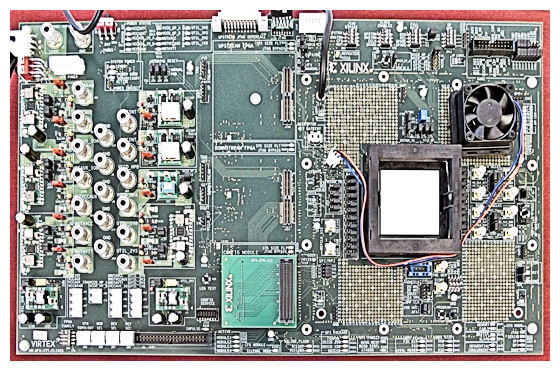
\includegraphics[height=60mm]{Figures/fpga.jpg}

% Title, author and degree
\vspace{0.8cm}
{\FontLb C Compiler for the VERSAT Reconfigurable Processor} \\
\vspace{3.6cm}
{\FontMb Gonçalo da Conceição Reis dos Santos} \\
\vspace{1.9cm}
{\FontLn Thesis to obtain the Master of Science Degree in} \\
\vspace{0.3cm}
{\FontLb Electrical and Computer Engineering} \\
%\vspace{1.9cm}
\vspace{1.0cm}
{\FontSn %
\begin{tabular}{ll}
Supervisor: & Prof. José João Henriques Teixeira de Sousa
\end{tabular} } \\
\vspace{1.0cm}
{\FontMb Examination Committee} \\
\vspace{0.3cm}
{\FontSn %
\begin{tabular}{ll}
Chairperson: & Prof. Francisco André Corrêa Alegria\\
Supervisor: & Prof. José João Henriques Teixeira de Sousa \\
Member of the Committee: & Prof. Paulo Ferreira Godinho Flores \\
\end{tabular} } \\
\vspace{1.5cm}
{\FontMb November 2019} \\
%
\end{center}

\cleardoublepage
 % file "Thesis_FrontCover.tex"
\cleardoublepage

% ----------------------------------------------------------------------
% Dedication page (optional)
% ----------------------------------------------------------------------
%%%%%%%%%%%%%%%%%%%%%%%%%%%%%%%%%%%%%%%%%%%%%%%%%%%%%%%%%%%%%%%%%%%%%%%%%
%                                                                      %
%     File: Thesis_Dedication.tex                                      %
%     Tex Master: Thesis.tex                                           %
%                                                                      %
%     Author: Andre C. Marta                                           %
%     Last modified :  2 Jul 2015                                      %
%                                                                      %
%%%%%%%%%%%%%%%%%%%%%%%%%%%%%%%%%%%%%%%%%%%%%%%%%%%%%%%%%%%%%%%%%%%%%%%%

\null\vskip5cm%
\begin{flushright}
     Dedicated to someone special...
\end{flushright}
\vfill\newpage

 % file "Thesis_Dedication.tex"
%\cleardoublepage

% ----------------------------------------------------------------------
%  Declaration
% ----------------------------------------------------------------------
\section*{Declaration}
I declare that this document is an original work of my own authorship and that it 
fulfills all the requirements of the Code of Conduct and Good Practices of the 
Universidade de Lisboa.
\cleardoublepage

% ----------------------------------------------------------------------
%  Acknowledgments (optional)
% ----------------------------------------------------------------------
%%%%%%%%%%%%%%%%%%%%%%%%%%%%%%%%%%%%%%%%%%%%%%%%%%%%%%%%%%%%%%%%%%%%%%%%
%                                                                      %
%     File: Thesis_Acknowledgments.tex                                 %
%     Tex Master: Thesis.tex                                           %
%                                                                      %
%     Author: Andre C. Marta                                           %
%     Last modified :  2 Jul 2015                                      %
%                                                                      %
%%%%%%%%%%%%%%%%%%%%%%%%%%%%%%%%%%%%%%%%%%%%%%%%%%%%%%%%%%%%%%%%%%%%%%%%

\section*{\acknowledgments}

% Add entry in the table of contents as section
\addcontentsline{toc}{section}{\acknowledgments}

I want to thank my supervisor, Professor José Teixeira de Sousa, for the 
opportunity to develop this work and for his guidance and support during that process. 
His help was fundamental to overcome the multiple obstacles that I faced during this work.

I also want to acknowledge Professor Horácio Neto for providing a simple Convolutional 
Neural Network application, used as a basis for the application developed for the 
RV32-Versat architecture.

A special acknowledgement goes to my friends, for their continuous support, and Válter,  
that is developing a multi-layer architecture for RV32-Versat. When everything seemed to 
be doomed he always had a miraculous solution.

Finally, I want to express my sincere gratitude to my family for giving me all the 
support and encouragement that I needed throughout my years of study and through the 
process of researching and writing this thesis. They are also part of this work.\\

\textbf{Thank you.}

 % file "Thesis_Acknowledgements.tex"
\cleardoublepage

% ----------------------------------------------------------------------
%  Abstract (both in English and Portuguese)
% ----------------------------------------------------------------------
\newacro{CGRA}{Coarse-Grain Reconfigurable Array}
\newacro{CPU}{Central Processing Unit}

%%%%%%%%%%%%%%%%%%%%%%%%%%%%%%%%%%%%%%%%%%%%%%%%%%%%%%%%%%%%%%%%%%%%%%%%
%                                                                      %
%     File: Thesis_Resumo.tex                                          %
%     Tex Master: Thesis.tex                                           %
%                                                                      %
%     Author: Carlos A. Rodrigues                                           %
%     Last modified : 21 Jan 2011                                      %
%                                                                      %
%%%%%%%%%%%%%%%%%%%%%%%%%%%%%%%%%%%%%%%%%%%%%%%%%%%%%%%%%%%%%%%%%%%%%%%%

\section*{Resumo}

% Add entry in the table of contents as section
\addcontentsline{toc}{section}{Resumo}

Inserir o resumo em Portugu\^{e}s aqui com o máximo de 250 palavras e acompanhado de 4 a 6 palavras-chave...

\vfill

\textbf{\Large Palavras-chave:} OpenRISC, Sistema em um chip,...

\cleardoublepage

   % file "Thesis_Resumo.tex"
\cleardoublepage

%%%%%%%%%%%%%%%%%%%%%%%%%%%%%%%%%%%%%%%%%%%%%%%%%%%%%%%%%%%%%%%%%%%%%%%%
%                                                                      %
%     File: Thesis_Abstract.tex                                        %
%     Tex Master: Thesis.tex                                           %
%                                                                      %
%     Author: Andre C. Marta                                           %
%     Last modified :  2 Jul 2015                                      %
%                                                                      %
%%%%%%%%%%%%%%%%%%%%%%%%%%%%%%%%%%%%%%%%%%%%%%%%%%%%%%%%%%%%%%%%%%%%%%%%

\section*{Abstract}

% Add entry in the table of contents as section
\addcontentsline{toc}{section}{Abstract}

Versat is a Coarse-Grain Reconfigurable Array architecture (CGRA), which
implements self and partial reconfiguration by using a simple controller
unit. This report studies the current state of the art in HDL and CGRA
simulation, providing a basis to the development of a simulation environment for
Versat. The main objective of this environment is to provide a faster way to
develop and debug software without the use of prototyping hardware. Therefore,
the two types of HDL simulators, event-driven and cycle-accurate, their
advantages and disadvantages are studied, along with a performance comparison
between them. A study of high-level implementations for CGRA simulation is
also presented.

\vfill

\textbf{\Large Keywords:} Versat, coarse-grain reconfigurable arrays, HDL
simulation, CGRA simulation, high-level simulation

 % file "Thesis_Abstract.tex"
\cleardoublepage

% ----------------------------------------------------------------------
%  Table of contents, list of tables, list of figures and nomenclature
% ----------------------------------------------------------------------

% Table of contents
%
\tableofcontents
\cleardoublepage 

% List of tables
%
% Add entry in the table of contents as section
\phantomsection
\addcontentsline{toc}{section}{\listtablename}
% Generate list
\listoftables
\cleardoublepage 

% List of figures
%
% Add entry in the table of contents as section
\phantomsection
\addcontentsline{toc}{section}{\listfigurename}
% Generate list
\listoffigures
\cleardoublepage 

\phantomsection
\chapter*{List of Acronyms}
% Add entry in the table of contents as section
\addcontentsline{toc}{section}{List of Acronyms}
%\begin{acronym}[CGRA]
\newacro{CGRA}{Coarse-Grain Reconfigurable Array}
\newacro{CPU}{Central Processing Unit}
\newacro{ISA}{Instruction Set Architecture}
\newacro{UART}{Universal Asynchronous Receiver-Transmitter}
\newacro{LED}{Light Emitting Diode}
\newacro{CM}{Configuration Module}
\newacro{DE}{Data Engine}
\newacro{FU}{Functional Units}
\newacro{AGU}{Address Generation Unit}
\newacro{LUT}{Lookup Tables}
\newacro{FPGA}{Field-Programmable Gate Array}
\newacro{ASIC}{Application-Specific Integrated Circuit}
\newacro{CPI}{Cycles Per Instruction}
\newacro{CNN}{Convolutional Neural Network}
\newacro{HDL}{Hardware Description Language}
\newacro{RTL}{Register-Transfer Level}
\newacro{UUT}{Unit Under Test}
\newacro{VPI}{Verilog Procedural Interface}
\newacro{API}{Application Programming Interface}
\newacro{DMA}{Direct Memory Access}
\newacro{VCD}{Value Change Dump}
\newacro{BRAM}{Block Random Access Memories}
\newacro{DSP}{Digital Signal Processor}
\newacro{ASIP}{Application Specific Instruction Set Processors}
\newacro{ALU}{Arithmetic Logic Unit}
%\end{acronym}
%print list

\noindent
\textbf{AGU} Address Generation Unit\\
\textbf{ALU} Arithmetic Logic Unit\\
\textbf{API} Application Programming Interface\\
\textbf{ASIC} Application-Specific Integrated Circuit\\
\textbf{ASIP} Application Specific Instruction Set Processor\\
\textbf{BRAM} Block Random Access Memory\\
\textbf{CGRA} Coarse-Grain Reconfigurable Array\\
\textbf{CM} Configuration Module\\
\textbf{CNN} Convolutional Neural Network\\
\textbf{CPI} Cycles Per Instruction\\
\textbf{CPU} Central Processing Unit\\
\textbf{DE} Data Engine\\
\textbf{DMA} Direct Memory Access\\
\textbf{DSP} Digital Signal Processor\\
\textbf{FPGA} Field-Programmable Gate Array\\
\textbf{FU} Functional Unit\\
\textbf{HDL} Hardware Description Language\\
\textbf{ISA} Instruction Set Architecture\\
\textbf{LED} Light Emitting Diode\\
\textbf{LUT} Lookup Table\\
\textbf{RTL} Register-Transfer Level\\
\textbf{UART} Universal Asynchronous Receiver-Transmitter\\
\textbf{UUT} Unit Under Test\\
\textbf{VCD} Value Change Dump\\
\textbf{VPI} Verilog Procedural Interface\\ % file "Thesis_Acronyms.tex"
\cleardoublepage

% Nomenclature
%
% entries of nomenclature list
%%%%%%%%%%%%%%%%%%%%%%%%%%%%%%%%%%%%%%%%%%%%%%%%%%%%%%%%%%%%%%%%%%%%%%%%%
%                                                                      %
%     File: Thesis_Nomenclature.tex                                    %
%     Tex Master: Thesis.tex                                           %
%                                                                      %
%     Author: Gonçalo Santos                                           %
%     Last modified : 20 Oct 2018                                      %
%                                                                      %
%%%%%%%%%%%%%%%%%%%%%%%%%%%%%%%%%%%%%%%%%%%%%%%%%%%%%%%%%%%%%%%%%%%%%%%%
%
% The definitions can be placed anywhere in the document body
% and their order is sorted by <symbol> automatically when
% calling makeindex in the makefile
%
% The \glossary command has the following syntax:
%
% \glossary{entry}
%
% The \nomenclature command has the following syntax:
%
% \nomenclature[<prefix>]{<symbol>}{<description>}
%
% where <prefix> is used for fine tuning the sort order,
% <symbol> is the symbol to be described, and <description> is
% the actual description.

% ----------------------------------------------------------------------
% Roman symbols [r]
\nomenclature[ru]{$\bf u$}{Velocity vector.}
\nomenclature[ru]{$u,v,w$}{Velocity Cartesian components.}
\nomenclature[rp]{$p$}{Pressure.}
\nomenclature[rC]{$C_D$}{Coefficient of drag.}
\nomenclature[rC]{$C_L$}{Coefficient of lift.}
\nomenclature[rC]{$C_M$}{Coefficient of moment.}

% ----------------------------------------------------------------------
% Greek symbols [g]
\nomenclature[g]{$\rho$}{Density.}
\nomenclature[g]{$\alpha$}{Angle of attack.}
\nomenclature[g]{$\beta$}{Angle of side-slip.}
\nomenclature[g]{$\mu$}{Molecular viscosity coefficient.}
\nomenclature[g]{$\kappa$}{Thermal conductivity coefficient.}

% ----------------------------------------------------------------------
% Subscripts [s]
\nomenclature[s]{$x,y,z$}{Cartesian components.}
\nomenclature[s]{$i,j,k$}{Computational indexes.}
\nomenclature[s]{$\infty$}{Free-stream condition.}
\nomenclature[s]{ref}{Reference condition.}
\nomenclature[s]{$n$}{Normal component.}

% ----------------------------------------------------------------------
% Supercripts [t]
\nomenclature[t]{T}{Transpose.}
\nomenclature[t]{*}{Adjoint.}

 % file "Thesis_Nomenclature.tex"
%
% Add entry in the table of contents as section
%\phantomsection
%\addcontentsline{toc}{section}{\nomname}
% Insert glossary/nomenclature section produced by MakeIndex
%\printnomenclature
%\cleardoublepage

% entries of glossary list
%%%%%%%%%%%%%%%%%%%%%%%%%%%%%%%%%%%%%%%%%%%%%%%%%%%%%%%%%%%%%%%%%%%%%%%%%
%                                                                      %
%     File: Thesis_Glossary.tex                                        %
%     Tex Master: Thesis.tex                                           %
%                                                                      %
%     Author: Carlos A. Rodrigues                                           %
%     Last modified : 30 Oct 2012                                      %
%                                                                      %
%%%%%%%%%%%%%%%%%%%%%%%%%%%%%%%%%%%%%%%%%%%%%%%%%%%%%%%%%%%%%%%%%%%%%%%%
%
% The definitions can be placed anywhere in the document body
% and their order is sorted by <symbol> automatically when
% calling makeindex in the makefile
%
% The \glossary command has the following syntax:
%
% \glossary{entry}
%
% The \nomenclature command has the following syntax:
%
% \nomenclature[<prefix>]{<symbol>}{<description>}
%
% where <prefix> is used for fine tuning the sort order,
% <symbol> is the symbol to be described, and <description> is
% the actual description.

% ----------------------------------------------------------------------

\glossary{name={\textbf{MDO}},description={Multi-Disciplinar Optimization is an engineering technique that uses optimization methods to solve design problems incorporating two or more disciplines.}}

\glossary{name={\textbf{CFD}},description={Computational Fluid Dynamics is a branch of fluid mechanics that uses numerical methods and algorithms to solve problems that involve fluid flows.}}

\glossary{name={\textbf{CSM}},description={Computational Structural Mechanics is a branch of structure mechanics that uses numerical methods and algorithms to perform the analysis of structures and its components.}}

 % file "Thesis_Glossary.tex"

% Add entry in the table of contents as section
%\phantomsection
%\addcontentsline{toc}{section}{\glossaryname}
% Insert glossary section produced by MakeIndex
%\printglossary
%\cleardoublepage

% Set arabic numbering (1,2,...) after preface
%
\setcounter{page}{1}
\pagenumbering{arabic}

% ----------------------------------------------------------------------
%  Chapters
% ----------------------------------------------------------------------

%%%%%%%%%%%%%%%%%%%%%%%%%%%%%%%%%%%%%%%%%%%%%%%%%%%%%%%%%%%%%%%%%%%%%%%%
%                                                                      %
%     File: Thesis_Introduction.tex                                    %
%     Tex Master: Thesis.tex                                           %
%                                                                      %
%     Author: Andre C. Marta                                           %
%     Last modified :  2 Jul 2015                                      %
%                                                                      %
%%%%%%%%%%%%%%%%%%%%%%%%%%%%%%%%%%%%%%%%%%%%%%%%%%%%%%%%%%%%%%%%%%%%%%%%

\chapter{Introduction}
\label{chapter:introduction}




In this report, the problem of accelerating the execution of Deep Neural
Networks (DNNs) using Coarse GRained Reconfigurable Arrays (CGRAs) is studied,
with special emphasis on compiling a DNN description into code that runs on
CPU/CGRA system. The Deep Versat Architecture~\cite{valter:deepversat} CGRA will be used as an
implementation tool in this work.


%%%%%%%%%%%%%%%%%%%%%%%%%%%%%%%%%%%%%%%%%%%%%%%%%%%%%%%%%%%%%%%%%%%%%%%%
\section{Problem}
\label{section:problem}

Neural Networks have been an object of study since the 1940's, but until the
beginning of this decade their applications were limited and did not play a
major role in computer vision conferences. With its meteoric rise in research,
several solutions to accelerate this algorithm have appeared, from Field Programmable Gate Arrays (FPGA) to
Application Specific Integrated Circuits (ASIC) implementations.

Convolutional Neural Networks (CNNs) are a particular kind of DNN where the output
values of the neurons in one layer are convolved with a kernel to produce the
input values of the neurons of the next layer. This algorithm is compute bound,
that is, its performance depends on how fast it can do certain calculations, and
depend less on the memory access time. Namely the convolutional layers take
approximately 90$\%$ of the computation time.

The acceleration of these workloads is a matter of importance for today's
applications such as image processing for object recognition or simply to
enhance certain images. Other uses like instant translation and virtual
assistants are applications of neural networks and their acceleration is of
vital importance to bring them into Internet of Things.

A suitable circuit to accelerate DNNs in hardware is the CGRA. A CGRA is a
collection of Functional Units and memories with programmable interconnections
in order to form computational datapaths. A CGRA can be implemented in both
FPGAs and ASICs. CGRAs can be reconfigured much faster than FPGAs, as they have
much less configuration bits. If reconfiguration is done at runtime, CGRAs add
temporal scalability to the spacial scalability that characterize
FPGAs. Moreover, partial reconfiguration is much easier to do in CGRAs compared
to FPGAs which further speeds up reconfiguration time. Another advantage of
CGRAs is the fact that they can be programmed entirely in software, contrasting
with the large development time of customized Intellectual Property (IP) blocks.
The Coarse Grain Reconfigurable Arrays (CGRA) is a midway acceleration solution
between FPGAs, which are flexible but large, power hungry and difficult to
reprogram, and ASICs, which are fast but generally not programmable.

However, mapping a specific DNN to a CGRA requires knowledge of its
architecture, latencies and register configurations, which may become a lengthy
process, especially if the user wants to explore the design space for several
DNN configurations. An automatic compiler that can map a standard DNN
description into CPU/CGRA code would dramatically decrease time to market of its
users. Currently there are equivalent tools for CPUs and GPUs and
even for FPGAS.


%%%%%%%%%%%%%%%%%%%%%%%%%%%%%%%%%%%%%%%%%%%%%%%%%%%%%%%%%%%%%%%%%%%%%%%%
\section{Solution}
\label{section:solution}

The proposed solution is a compiler that takes a configuration file from a
neural network framework like Caffe or Darknet. This new tool inputs the
parameters of Deep Versat, such as the number of layers and functional units,
and produces the C code needed for the Versat runs. This code is run on the
RISC-V picorv32~\cite{picorv} CPU controller that has Deep Versat as a peripheral.

%%%%%%%%%%%%%%%%%%%%%%%%%%%%%%%%%%%%%%%%%%%%%%%%%%%%%%%%%%%%%%%%%%%%%%%%
%\section{Thesis Outline}
%\label{section:outline}

%Briefly explain the contents of the different chapters...

%%%%%%%%%%%%%%%%%%%%%%%%%%%%%%%%%%%%%%%%%%%%%%%%%
%\section{Author's Work}
%\label{section:authorwork}

%TO ADD----

%%%%%%%%%%%%%%%%%%%%%%%%%%%%%%%%%%%%%%%%%%%%%%%%%%
\section{Report Outline}
\label{reportoutline}

This report is composed of 4 more chapters. In the second chapter, the
state-of-the-art of neural networks and the difficulties accelerating them is
described. In the third chapter, the Deep Versat architecture and how to program
it is explained. In the fourth chapter, CNN compiler techniques are
explored. Finally, the last chapter contains the proposed solution and the plan
for its execution.


 % file "Thesis_Introduction.tex"
\cleardoublepage

%%%%%%%%%%%%%%%%%%%%%%%%%%%%%%%%%%%%%%%%%%%%%%%%%%%%%%%%%%%%%%%%%%%%%%%%
%                                                                      %
%     File: Thesis_Versat.tex                                      %
%     Tex Master: Thesis.tex                                           %
%                                                                      %
%     Author: Andre C. Marta                                           %
%     Last modified :  2 Jul 2015                                      %
%                                                                      %
%%%%%%%%%%%%%%%%%%%%%%%%%%%%%%%%%%%%%%%%%%%%%%%%%%%%%%%%%%%%%%%%%%%%%%%%

\chapter{The Versat architecture}
\label{chapter:versat}

\begin{figure}[!htb]
	\centering
	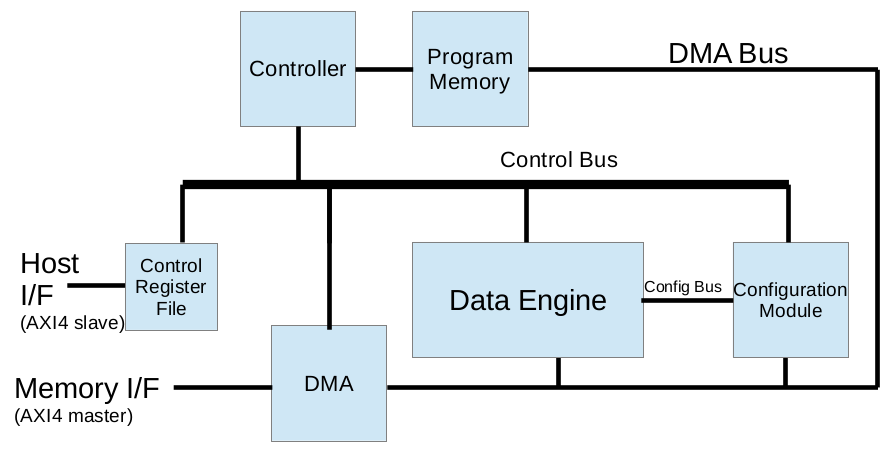
\includegraphics[width=0.8\textwidth]{Figures/top.png}
	\caption{Versat top-level entity.}
	\label{fig:top}
\end{figure}

The Versat architecture~\cite{sousa:versat, sousa:versat2016, sousa:controller,
  sousa:compiler} is shown in Figure~\ref{fig:top}, and it consists of the
following modules: Controller, Program Memory, Control Register File, DMA, Data
Engine and Configuration Module. The Controller can access the various modules
in the system via the Control Bus, and it executes programs stored in the
Program Memory (9kB = 1kB boot ROM + 8kB RAM). The user programs are loaded in
the RAM to execute algorithms which involve managing Data Engine (DE)
reconfigurations and DMA data transfers.

Versat user programs can use the DE to carry out data intensive computations. To
perform these computations, the Controller writes DE configurations to the
Configuration Module (CM) or simply restores configurations previously stored in
the CM. The Controller can also load the DE with data to be processed or save
the processed data back in the external memory using the DMA engine. The DMA
engine can also be used to initially load the Versat program or to move CGRA
configurations between the core and the external memory.

The Versat core has a host and a memory interface. Both of them use ARM’s
Advanced eXtensible Interface (AXI), a standard for busing. The host interface
(AXI slave) is used by a host system to instruct Versat to load and execute
programs. The host and the Controller communicate using the Control Register
File (CRF), an unit that is also used by Versat programs as a general purpose
(1-cycle access) register file. The memory interface (AXI master) is used to
access data from an external memory using the DMA.



%%%%%%%%%%%%%%%%%%%%%%%%%%%%%%%%%%%%%%%%%%%%%%%%%%%%%%%%%%%%%%%%%%%%%%%%
\section{Data Engine}
\label{section:data}

\begin{figure}[!htb]
	\centering
	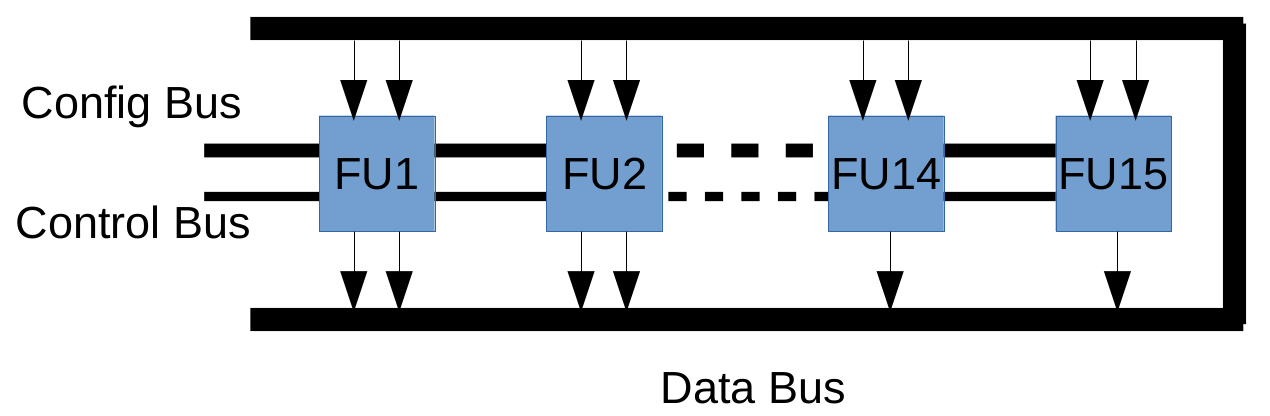
\includegraphics[width=0.8\textwidth]{Figures/de.png}
	\caption{Versat data engine.}
	\label{fig:de}
\end{figure}

The Data Engine (DE) has a flexible topology, in which the user can configure
the amount of functional units (FUs) and their respective type. In
Figure~\ref{fig:de} is shown a DE example with 15 FUs. The DE is a 32-bit
architecture with the following configurable FUs: Arithmetic and Logic Unit
(ALU), Multiplier Accumulator (MAC), Barrel Shifter (BS) and dual-port 16kB
embedded memories (MEM). The output registers of the FUs are read/write
accessible by the Controller via the Control Bus.

The FUs are interconnected by a wide bus called the Data Bus. This bus is the
concatenation of all FU outputs, with each FU contributing with a 32-bit section
to the Data Bus. An embedded memory contributes 2 sections to the Data Bus,
since it has 2 ports. These sections can be selected by each FU, according to
the configurations that they receive from the respective configuration registers
in the CM, whose outputs are concatenated in another wide bus called the Config
Bus.

The DE has a full mesh topology, meaning that each FU can select any FU output
as one of its inputs. This kind of structure may seem unnecessary but it greatly
simplifies the compiler design as it avoids expensive place and route
algorithms~\cite{sousa:versat2016}.

\begin{figure}[!htb]
	\centering
	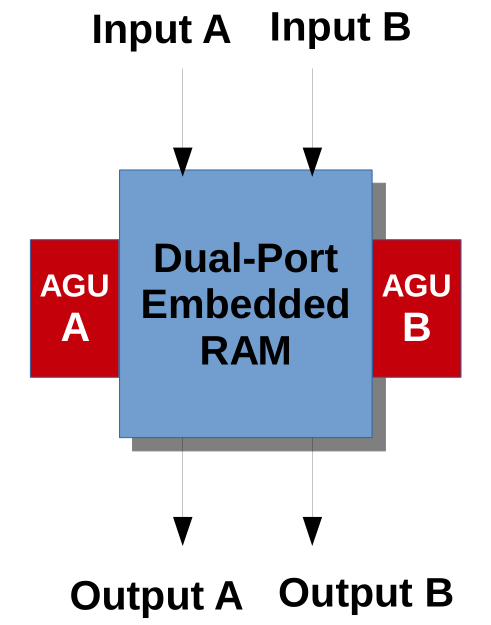
\includegraphics[width=0.23\textwidth]{Figures/memory.png}
	\caption{Versat dual-port embedded memory with AGUs.}
	\label{fig:memory}
\end{figure}

Each one of the dual-port memories used in Versat have a data input, a data
output and an address input, as shown in Figure~\ref{fig:memory}. Also, each
port has an Address Generation Unit (AGU), that can be programmed to generate
the address sequence used to access data from the memory port during the
execution of a program loop in the DE. The AGUs support two levels of nested
loops and can start execution with a programmable delay, so that circuit paths
with different latencies can be synchronized.

%%%%%%%%%%%%%%%%%%%%%%%%%%%%%%%%%%%%%%%%%%%%%%%%%%%%%%%%%%%%%%%%%%%%%%%%
\section{Configuration Module}
\label{section:configuration}

\begin{figure}[!htb]
	\centering
	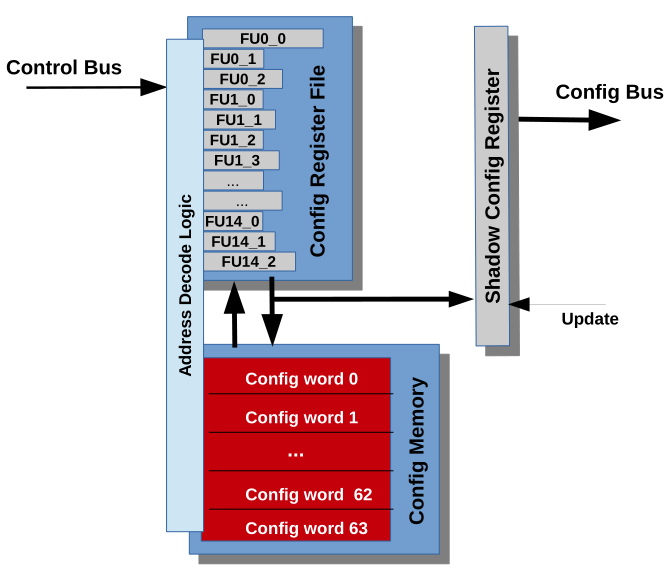
\includegraphics[width=0.6\textwidth]{Figures/configuration.png}
	\caption{Versat configuration module example.}
	\label{fig:cm}
\end{figure}

In Versat, the configuration bits are organized in configuration spaces, one for
each FU. Each configuration space comprises multiple fields, which are memory
mapped from the Controller point of view. Thus, the Controller is able to change
a single configuration field of an FU by writing to the respective address. This
implements partial reconfiguration.

A Configuration Module (CM) example is illustrated in Figure~\ref{fig:cm}, with
a reduced number of configuration spaces and fields for simplicity. It contains
a register file with a variable length (the length depends on the FUs used), a
shadow register and a memory. The shadow register holds the current
configuration of the DE, which is copied from the main configuration register
whenever the Update signal is activated. This means that the configuration
register can be changed in the main register while the DE is running.

When the CM is addressed by the Controller, the decode logic checks if the
configuration register file or the configuration memory is being addressed. The
configuration register file accepts write requests and ignores read requests. On
the other hand, the configuration memory deals with read and write requests in
the following way: a read request causes the addressed contents of the
configuration memory to be transferred into the configuration register file,
while a write request causes the contents of the configuration register file to
be stored into the addressed position of the configuration memory. This is a
mechanism for saving and loading entire configurations in a single clock cycle
because all the data transfers are internal.

%%%%%%%%%%%%%%%%%%%%%%%%%%%%%%%%%%%%%%%%%%%%%%%%%%%%%%%%%%%%%%%%%%%%%%%%
\section{Controller}
\label{section:controller}

\begin{figure}[!htb]
	\centering
	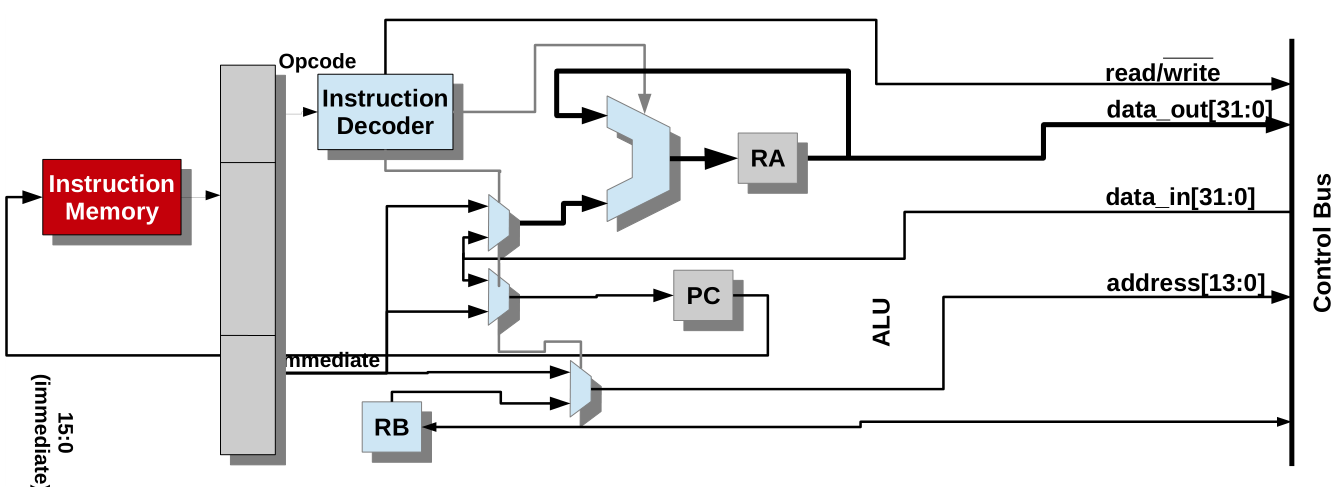
\includegraphics[width=0.8\textwidth]{Figures/controller.png}
	\caption{Versat controller.}
	\label{fig:controller}
\end{figure}

The controller used in the Versat architecture is just used for reconfiguration,
data transfer and simple algorithmic control. This controller is not meant to
replace a more general host processor, which can run complex applications while
using Versat as an accelerator.

The controller has an accumulator architecture, using a 2 stage pipeline, as
shown in Figure~\ref{fig:controller}. In this architecture 3 main registers are
used: RA, RB and PC. The RA is the accumulator, the RB is the address register,
used for indirect loads and stores, and the PC is the register that holds the
value of the program counter.

The controller is the master of a simple bus called the Control Bus, which can
be accessed using the 4 signals shown in Figure~\ref{fig:controller}. Register
RB can be accessed using the Control Bus as if it were a peripheral of the
Control Bus.

\begin{table}[!htbp]
	\centering
	\caption{Versat instruction set.}
	\label{tab:isa}
	\begin{tabular}{|c|l|}
		\hline 
		{\bf Mnemonic} & {\bf Description} \\
		\hline \hline 
		rdw & RA = (Imm)\\
		\hline
		wrw & (Imm) = RA\\
		\hline
		rdwb & RA = (RB)\\
		\hline
		wrwb & (RB) = RA\\
		\hline
		ldi & RA = Imm\\
		\hline
		ldih & RA[31:16] = Imm\\
		\hline
		beqi & RA == 0? PC = Imm: PC += 1; RA = RA-1\\
		\hline
		beq & RA == 0? PC = (Imm): PC += 1; RA = RA-1\\
		\hline
		bneqi & RA != 0? PC = Imm: PC += 1; RA = RA-1\\
		\hline
		bneq & RA != 0? PC = (Imm): PC += 1; RA = RA-1\\
		\hline
		add & RA = RA + (Imm)\\
		\hline
		addi & RA = RA + Imm\\
		\hline
		sub & RA = RA - (Imm)\\
		\hline
		shft & RA = (Imm $<$ 0)? RA=RA$<<$1: RA=RA$>>$1\\
		\hline
		and & RA = RA \& (Imm)\\
		\hline
		xor & RA = RA \^ (Imm)\\
		\hline
	\end{tabular}
\end{table}

The Versat controller Instruction Set Architecture (ISA) has 16 instructions, as
shown in Table~\ref{tab:isa}. Currently, it can only be programmed in assembly
language as it does not yet have a C compiler which is being developed by
another student working in this project.


%%%%%%%%%%%%%%%%%%%%%%%%%%%%%%%%%%%%%%%%%%%%%%%%%%%%%%%%%%%%%%%%%%%%%%%%
\section{Application Example}
\label{section:application}

During the work carried out for this report an application for an international
client using the Versat architecture was developed. It consists of an MP3
encoder, shown in Figure~\ref{fig:application}, where Versat is used to
accelerate the front end of the algorithm, denoted MP3-FE in
Figure~\ref{fig:application}).

\begin{figure}[!htb]
	\centering
	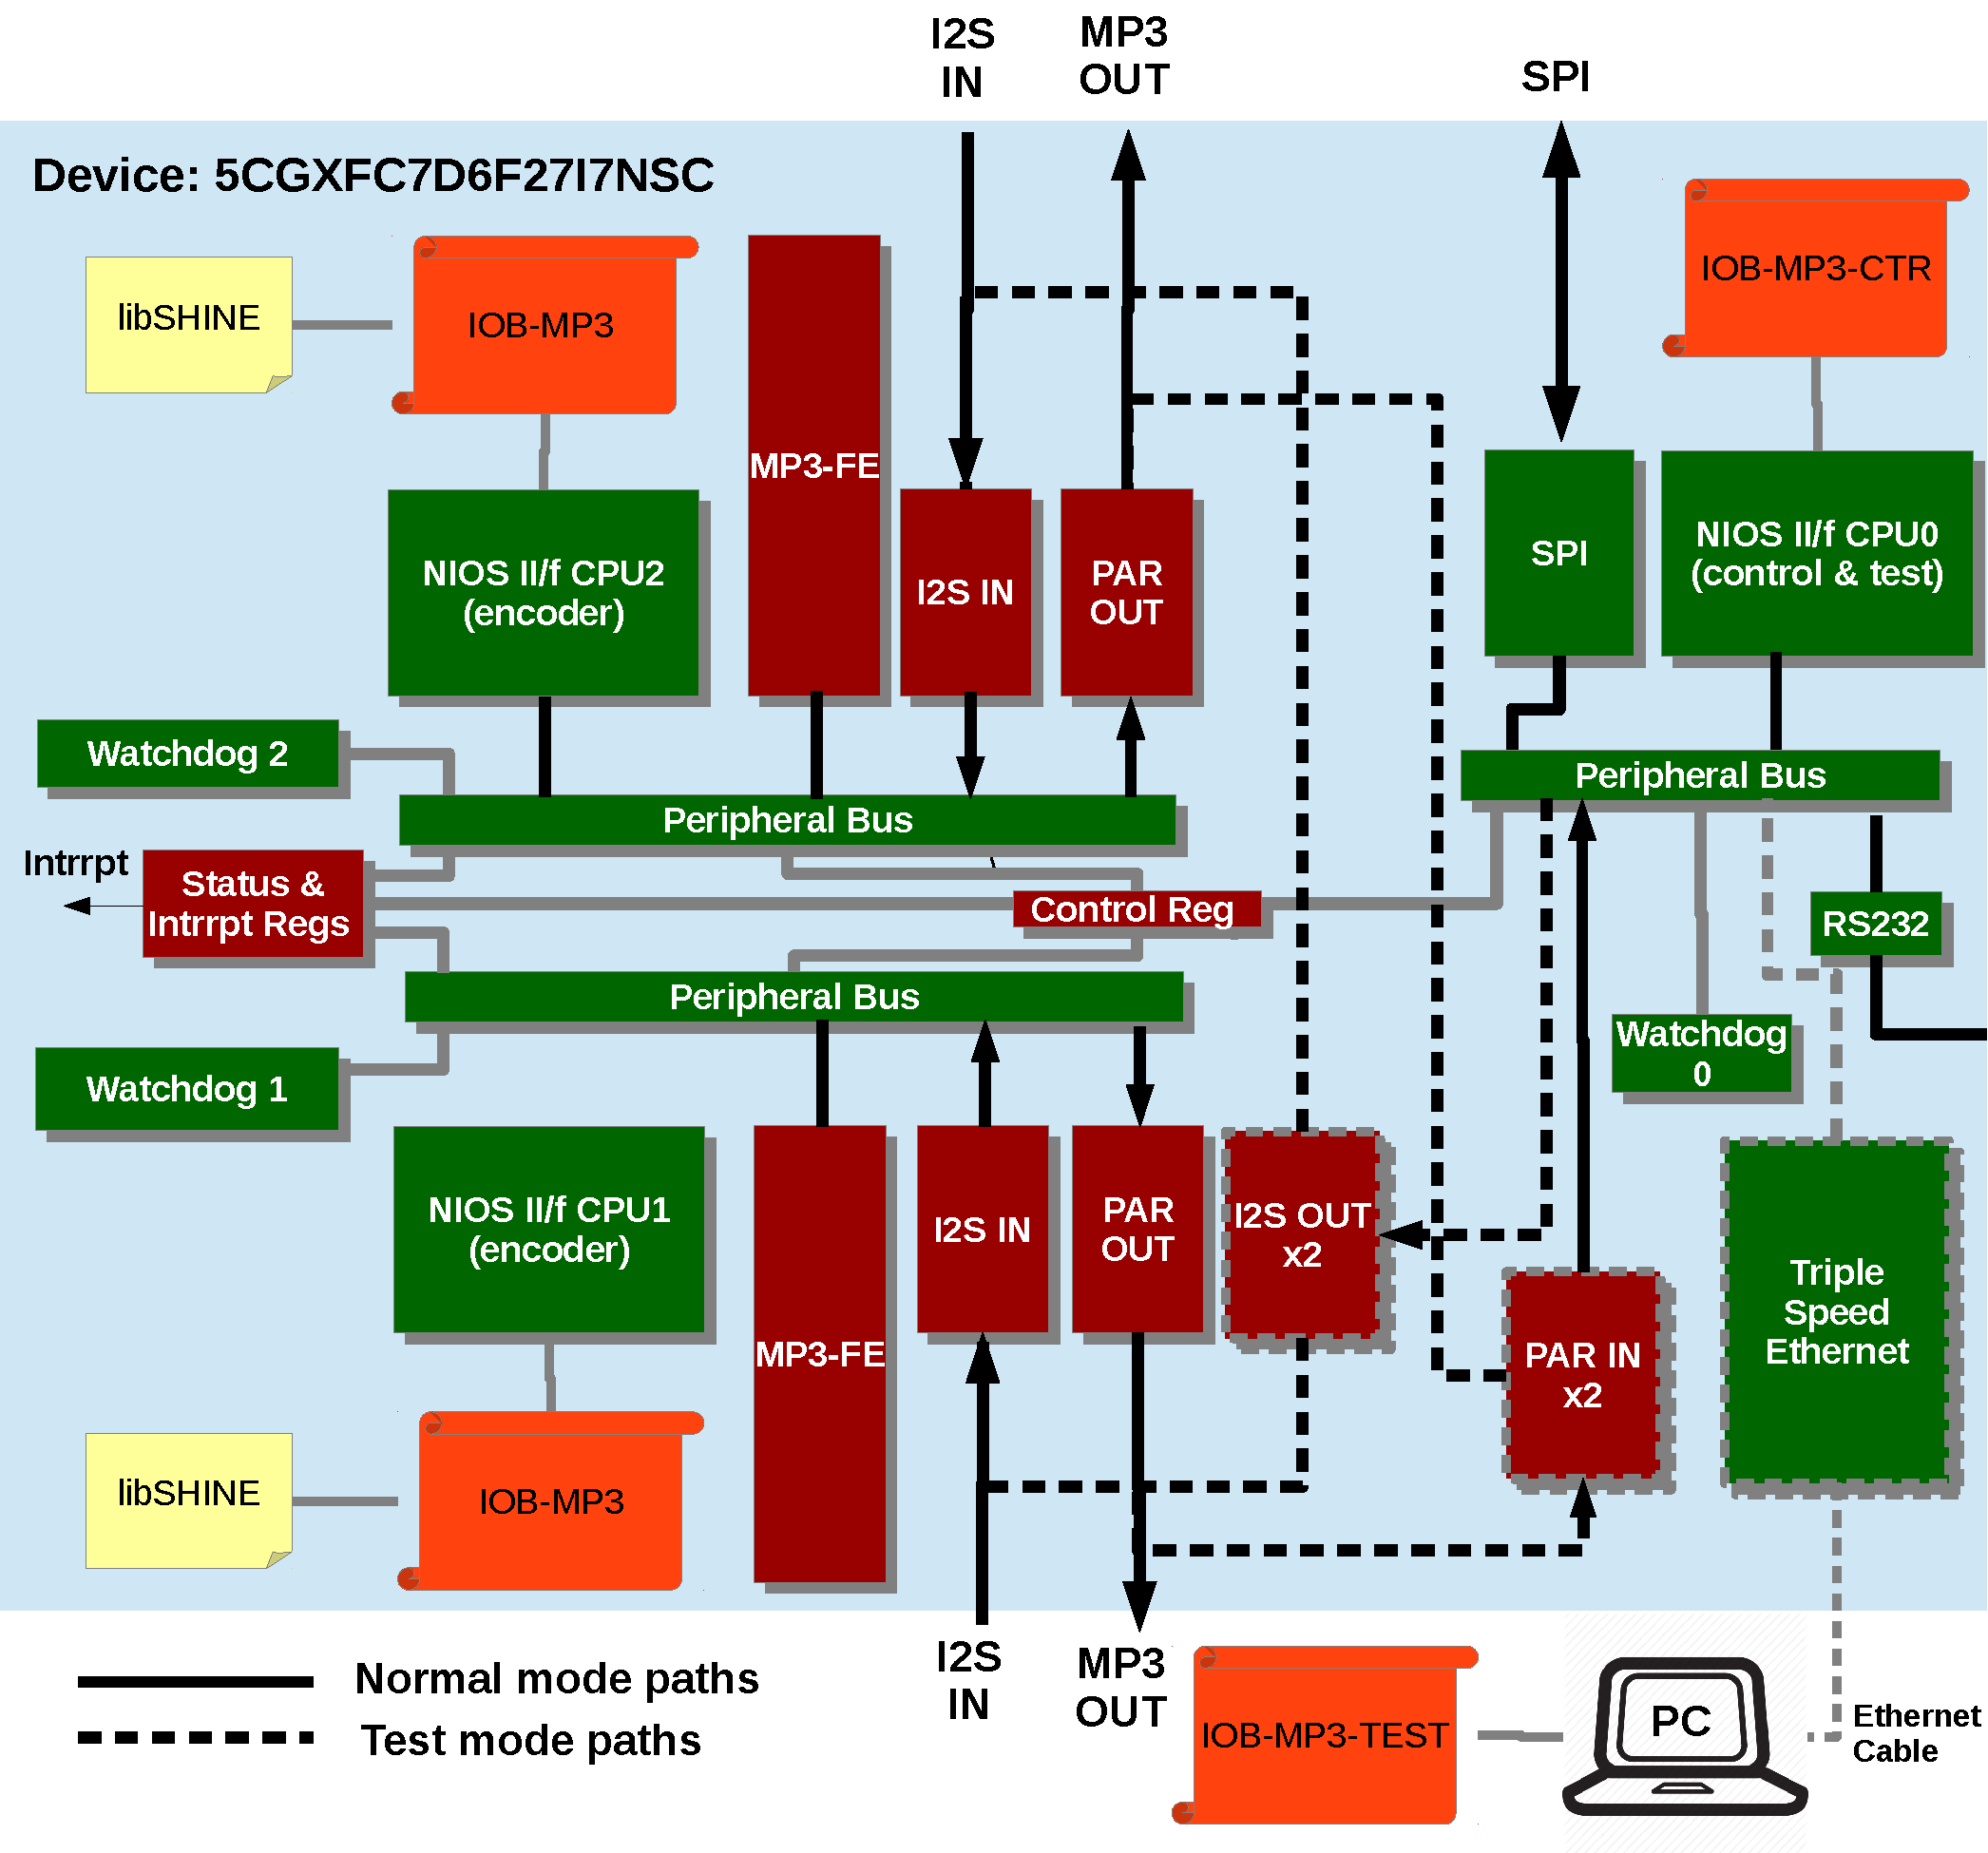
\includegraphics[width=0.85\textwidth]{Figures/bd.pdf}
	\caption{Schematic of the application where Versat was used.}
	\label{fig:application}
\end{figure}

The MP3 algorithm is based in Shine~\cite{shine:mp3}, a fast fixed-point MP3
encoding library. The front end runs sub-band filtering of the audio signal and
applies the Modified Discrete Cosine Transform to the result. These functions
are the most computationally expensive functions in the MP3 algorithm and
normally require DSP extensions to the ISA of the processor used. In the
approach taken, a more modest processor was used (Intel's NIOS2) which used
Versat as a peripheral acceleration core.

To run this algorithm the Versat architecture was configured with 4 dual-port
memories and 3 FUs: a Multiply Accumulate Unit (MAC), a simple Arithmetic and
Logic Unit (ALU) and a Barrel Shifter Unit (BS). The MP3 front-end was written
in the Versat Assembly language, since Versat compiler does not support yet the
use of a higher level programming language (like C or C++).

The FE was intensively simulated before synthesis and implementation in the
FPGA. Initially, the simulations were performed using Icarus
Verilog~\cite{icarus:verilog}, an open-source Verilog simulator. However, as the
complexity of the core increased, the simulation times also increased
dramatically, since Icarus Verilog is a fairly slow simulator, as will be seen
in section~\ref{section:performance}, where the performance of the different HDL
simulators is analysed.

As a result, at a certain point in the project, the simulator was changed to
Cadence NCSim~\cite{cadence:ncsim} to speed up the simulations. Despite NCsim
being considerably faster than Icarus Verilog, the simulations still took a
considerable amount of time. This reinforces the need for a faster simulation
environment for the Versat architecture.
 % file "Thesis_Versat.tex"
\cleardoublepage

%%%%%%%%%%%%%%%%%%%%%%%%%%%%%%%%%%%%%%%%%%%%%%%%%%%%%%%%%%%%%%%%%%%%%%%%
%                                                                      %
%     File: Thesis_Versat.tex                                          %
%     Tex Master: Thesis.tex                                           %
%                                                                      %
%     Author: Andre C. Marta                                           %
%     Last modified :  2 Jul 2015                                      %
%                                                                      %
%%%%%%%%%%%%%%%%%%%%%%%%%%%%%%%%%%%%%%%%%%%%%%%%%%%%%%%%%%%%%%%%%%%%%%%%

\chapter{HDL Simulators}
\label{chapter:simulators}

As mentioned before, HDL simulators play a fundamental role during the different
phases of circuit development, and there are multiple simulation tools that can
be used. However, despite all these tools having more or less the same purpose
(provide a way to validate the circuit being tested), they do not work in the
same way.

Typically, before testing a circuit, a test bench is created. The test bench is
a program, written in a HDL or in a programming language (like SystemC, for
example), that comprises three modules~\cite{tan:vhstas}: stimuli generator,
golden response generator and response analyser, as shown in
Figure~\ref{fig:tb}. The stimuli generator module is responsible for generating
the signals needed to make the circuit work properly. On the other hand, the
golden response generator computes the expected circuit response, based on the
inputs generated by the stimuli generator. Finally, the response analyzer
compares the circuit output signals with the ones generated by the golden
response generator. During simulation, if both signs are equal, it means that
the circuit is working as intended.

\begin{figure}[!htb]
	\centering
	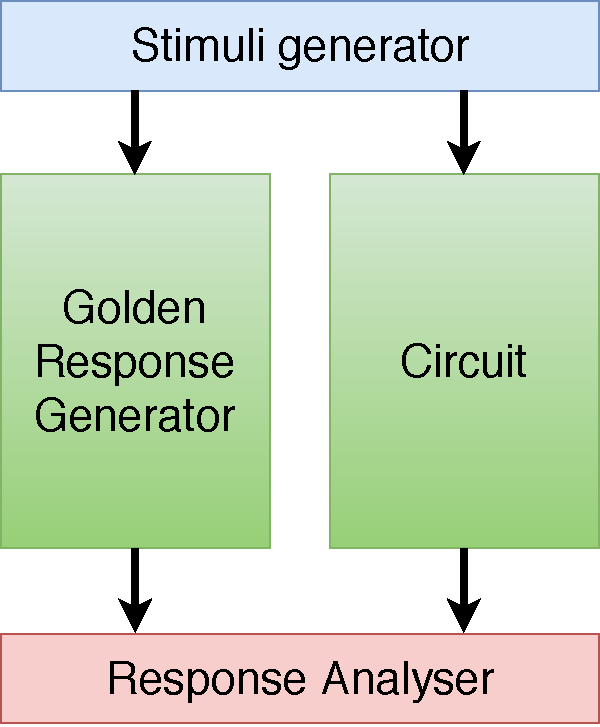
\includegraphics[width=0.42\textwidth]{Figures/Testbench.pdf}
	\caption{Test bench diagram.}
	\label{fig:tb}
\end{figure}

The results provided by the test-bench might depend on the chosen
simulator. This happens because all the simulators work in different ways: while
some focus on obtaining the most complete results (including simulation
timings), sacrificing the speed of the simulations, others do the opposite. In
this perspective, the simulators can be divided into two main categories~\cite{tan:vhstas,palnitkar:verilog}: event-driven or cycle-accurate.

\section{Event-Driven Simulators}
\label{section:event}

The first category of simulators are the event-driven
ones~\cite{tan:vhstas,gunes:survey,palnitkar:verilog}. This simulators work by
taking events sequentially, propagating them through the circuit until it
reaches a steady state.

The events are generated each time that a circuit input is changed, being stored
in a queue, ordered chronologically to allow the correct execution of the
events. When an event is evaluated, only the circuit nodes that have their input
changed by that event are evaluated. After evaluation, the event is removed from
the queue, with new events resultant from the output changes being added. This
means that the same element might be evaluated multiple times during the same
time step due to the feedback from some signals.

It's important to mention that during the simulation process there's a timer
that is used to keep track of the events timings. This leads to one of the main
advantages of event-driven simulation, which is the accurate simulation results,
with detailed timing information, allowing the identification of timing problems
in the tested circuit.

Despite this important advantage, this type of simulation also brings some
disadvantages, mainly related with its speed. Due to their complex algorithms
used for event scheduling and timing evaluation, event-driven simulators are
slow. While for relatively small circuits this might not be a significant
problem, for large circuits this is an important disadvantage, because their
increased complexity will increase significantly the simulation duration.

This type of simulators can be divided into 2 main categories: software or
hardware based, each one with different subcategories. These categories are
analysed in the following subsections.

\subsection{Software-based Simulators}
\label{subsection:software}

The software-based simulators are the most common type of simulators, including
simulators like the Cadence NCSim~\cite{cadence:ncsim}, the Synopsys
VCS~\cite{synopsys:vcs}, the Mentor Graphics ModelSim~\cite{mentor:modelsim} or
the Icarus Verilog~\cite{icarus:verilog}. Usually, they run on a general purpose
computer, being divided into three categories, according to their algorithms:
compiled-code, interpreter and gate level.

An interpreter software simulator reads the HDL code to simulate and interprets
it, translating the original code to a set of instructions accepted by the
simulator program. This translation process occurs during runtime and implies
the creation of data structures to store the data taken from the HDL file, that
will be used afterwards to create the simulation. This simulators are somewhat
inefficient, due to the resultant overhead of the code translation. This
typically results in the execution of a considerable number of instructions per
element evaluation, of which only a few perform logic model evaluation~\cite{lewis:compiled}.

On the other hand, a compiled-code simulator works by transforming the HDL
circuit description, including its testbench, into an equivalent C code (or some
similar programming language). The generated code is then compiled by a generic
complier (like gcc, for example), resulting in an executable file, that will the
be executed to run the simulation. This type of simulators are more efficient
than the interpreter ones, since they eliminate the overhead of traversing the
network data structures~\cite{lewis:compiled}. The most used simulators, like
Cadence NCSim, Synopsys VCS or Icarus Verilog belong to this category of
simulators.

Although the gate level simulators are either of the interpreted or
compiled-code type, they differ from the simulators referred in those
categories~\cite{tan:vhstas}. This happens because, while those simulators have
full Verilog compliance (supporting also gate level simulations), the gate level
simulators just support a small subset of Verilog.

RTL simulation is the most used method for circuit verification due to its
reasonable accuracy~\cite{sousa:reconfigurable}. However, in the last few years
there has been a rising trend in the industry to run gate level
simulations~\cite{khandelwal:gatelevel}. This happens mainly due to the more
complex timing checks required by modern process nodes. As a result, despite
gate level simulation being more time consuming than RTL simulation, it greatly
improves the verification results.

Usually, gate level simulation is used before going into the last stages of
circuit production. As shown in Figure~\ref{fig:gl},the circuit is synthesized
to a gate level netlist only after the RTL description of the circuit is working
properly. Then, the gate level netlist is simulated, with its results being
compared with the ones obtained with the RTL description. It they are equal,
then the circuit is working as intended.

\begin{figure}[!htb]
	\centering
	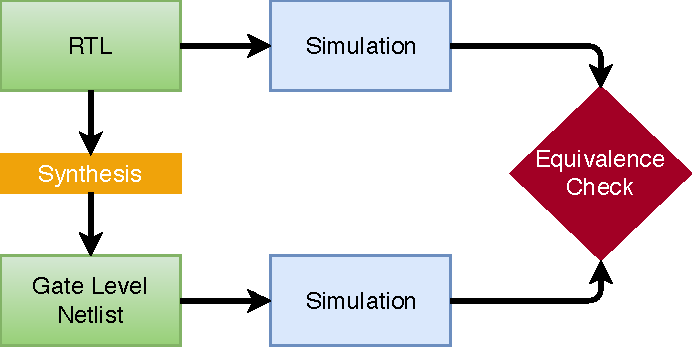
\includegraphics[width=0.7\textwidth]{Figures/Gate-level.pdf}
	\caption{Gate level design flow diagram.}
	\label{fig:gl}
\end{figure}

\subsection{Hardware-based Simulators}
\label{subsection:hardware}

As the name indicates, hardware-based simulators are a type of simulators that
rely on configurable hardware to do the digital circuit verification. When
compared with the software-based simulators, they have the advantage of being a
few orders of magnitude faster~\cite{tan:vhstas}. However they also have some
disadvantages: the hardware can be costly sometimes (depending on its
specifications) and it requires long compilation times, which makes them
needless for smaller designs. These simulators also require proprietary hardware
platforms to perform the desired simulations, with the hardware setup depending
on the platforms used, being different on each platform. As a result, these type
of simulators have a steep learning curve.

In this simulation type, the Verilog design is mapped onto a reconfigurable
piece of hardware with the same logical behavior as the netlist.  The simulation
is divided between the software simulator, which simulates all the Verilog code
that is not synthesizable, and the hardware accelerator, which simulates
everything that is synthesizable~\cite{khandelwal:gatelevel}. The design is then
run on the hardware, producing the simulation results. The results, like in a
Software-based simulator, must be checked in order to assess if the circuit is
working properly.

There are two variants of Hardware-based simulators: FPGA-based or
emulator-based. On one hand, the FPGA-based simulators, as the name indicates,
rely on FPGAs. A FPGA (Field Programmable Gate Array) is an integrated circuit
designed to be configured multiple times, according to the user needs. It
comprises an array of programmable logic blocks, memory elements, arithmetic
functions, etc.

The FPGA-based simulators follow the flow shown in Figure~\ref{fig:fpga}. The
original Verilog description of the code is transformed into an intermediate
representation, independent of the target platform. Here, the synthesizable
portions of the code are mapped into the FPGA, while the non synthesizable
portions (namely intendend for verification purposes) are run as software in the
host machine (software/hardware co-simulation). The simulator and the FPGA
interact with each other to produce the results.

\begin{figure}[!htb]
	\centering
	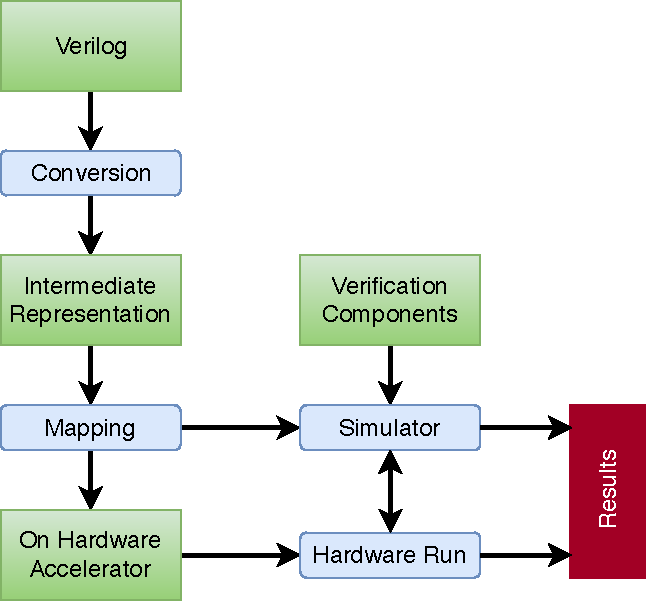
\includegraphics[width=0.7\textwidth]{Figures/FPGAsim.pdf}
	\caption{FPGA-based simulation flow~\cite{khandelwal:gatelevel}.}
	\label{fig:fpga}
\end{figure}

On the other hand, Emulator-based simulators rely on emulators to run their
simulations. An emulator is a specialized piece of hardware, that is , an
Application Specific Circuit (ASIC) that, when compared to a FPGA offers limited
reconfigurability, but with the advantage of a higher simulation speed. Even
though, the FPGA can run the actual circuit which in many cases superseeds
emulators in performance despite the lower clock frequency.

This type of simulation offers the possibility of testing software on the
developed design before having it implemented on chip, in a way that the
software application runs exactly as it would on the real chip in a real
circuit. It also offers the possibility for testing more complex programs, that
would take large amounts of time (sometimes even days) to run on other types of
simulators (like the software-based ones).

The simulation flow for this type of simulators has some similarities with the
FPGA-based simulators. In this case, as shown in Figure~\ref{fig:emulator}, the
Verilog code is converted into an intermediate representation, that will the be
mapped into the emulator. The code to be mapped must include only code that can
be implemented into the emulator. This means that the non synthesizable code
must be separated, being included in the software application. Both the software
and hardware platform interact with each other to produce the results.

\begin{figure}[!htb]
	\centering
	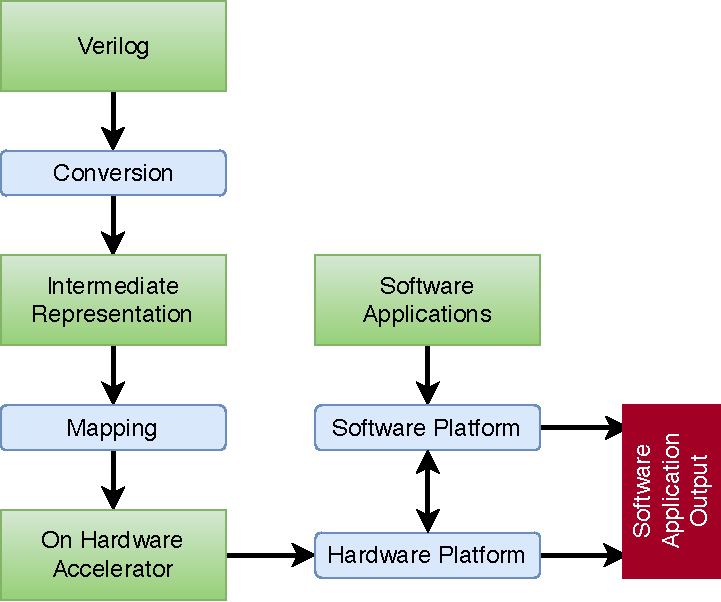
\includegraphics[width=0.7\textwidth]{Figures/Emulatorsim.pdf}
	\caption{Emulator-based simulation flow~\cite{khandelwal:gatelevel}.}
	\label{fig:emulator}
\end{figure}

\section{Cycle-Accurate Simulators}
\label{section:cycle}

Cycle-Accurate simulators are another important category of HDL
simulators. Instead of taking events sequentially, propagating them through the
circuit until it reaches a steady state, like the event-driven simulators, this
type of simulators evaluate each logic element of the circuit in a clock
cycle. They do this evaluation for each clock cycle, without taking into
consideration the propagation times and delays within the
cycle~\cite{khandelwal:gatelevel}.

As a result, these simulators are considerably faster than the event-driven
ones. However, they provide incomplete information about the circuit, since they
do not evaluate the delays and propagation times when evaluating each clock
cycle. So, if a circuit has timing problems, a cycle-accurate simulator will not
be able to notice them, making necessary the use of an even-driven simulator at
some stage to evaluate the existence of timing problems. All these
characteristics make the cycle-accurate simulators best suited for large circuit
simulation, like CPUs, when simulation speed is an important factor.

Most cycle-accurate simulators use a 2-state model (0 or 1) to calculate the
values of the signals through the circuit. A typical event-driven simulator uses
a more complex model, with more states (adding states like undefined, unknown or
high-impedance)~\cite{bennett:verilator}. This means that cycle-accurate
simulators have to make assumptions when the signals may have a value different
from 0 or 1 (for example, a signal that was uninitialized). While this speeds up
the simulation process, it also might be prone to produce wrong results.

From all the cycle-accurate simulators available, the most used one is probably
Verilator. Verilator is an open source simulator that compiles synthesizable
Verilog RTL, generating cycle accurate C++ and SystemC models. For each circuit, Verilator compiles a different model. These models are
then linked to a test bench, being executed in order to generate the
simulation. Verilator does not only translate Verilog code to C++ or
SystemC. Instead, it compiles the code into a much faster optimized and
thread-partitioned model, which is in turn wrapped inside a C++/SystemC
module~\cite{veripool:verilator}.

\section{Performance Comparison}
\label{section:performance}

When comparing event-driven and cycle-accurate simulators, not only their
working principles differ, but also their performance. Event-driven simulators
are typically slower than cycle-accurate simulators. This happens because the
algorithms used are more complex in event-driven simulators, having to implement
event scheduling and timing evaluation. The events are taken sequentially, being
propagated through the circuit until it reaches a steady state. New events
resultant from the output changes are added, meaning that the same element might
be evaluated multiple times during the same time step due to the feedback from
some signals. This whole process requires a considerable amount of time (and
computational power), being the main reason behind the lower speed of
event-driven simulators, when compared with cycle-accurate simulators.

The cycle-accurate simulators are typically the fastest type of simulators. This
happens because the simulation algorithm is simpler, evaluating each logic
element of the circuit in a clock cycle only once. They do this evaluation for
each clock cycle, without taking into consideration the propagation times and
delays within the cycle. There are also some simplifications that help improving
the simulation speed, like the use of a 2-state model (0 or 1) to calculate the
values of the signals through the circuit, instead of a model with multiple
states~\cite{bennett:verilator}.

In Figure~\ref{fig:performance} a graphic comparing the performance of the most
popular HDL simulators available in the market~\cite{verilator:benchmarks} is
shown. To run these benchmarks, a slightly modified model of the Motorolla M68K
processor was used. All the simulators shown were run in a general purpose
computer with an AMD Phenom 9500 2.2GHz processor, DDR2 667 Memory and running
the SuSE 11.1 operating system. The benchmark measures the number of cycles that
a simulator can run in a fixed amount of time, so a higher result means that
the simulator has a better performance.

From the analysis of the benchmark results, it can be concluded that Verilator
is considerably faster than the other tested simulators, both in 32 and 64 bits
versions. Cadence NCSim is almost 2 times slower than Verilator, while Synopsis
VCS is 3.5 times slower. Icarus Verilog is the slowest simulator tested, being
almost 80 times slower than Verilator. The benchmark results shown should only
work as reference, given their limitations: the versions of the simulators used
are already outdated, the same happening with the hardware and operating systems
used in the general purpose computers. Also, this benchmark only evaluates the
performance in one model (Motorolla M68K processor), instead of using multiple
models in order to provide more accurate results.

\begin{figure}[!htb]
	\centering
	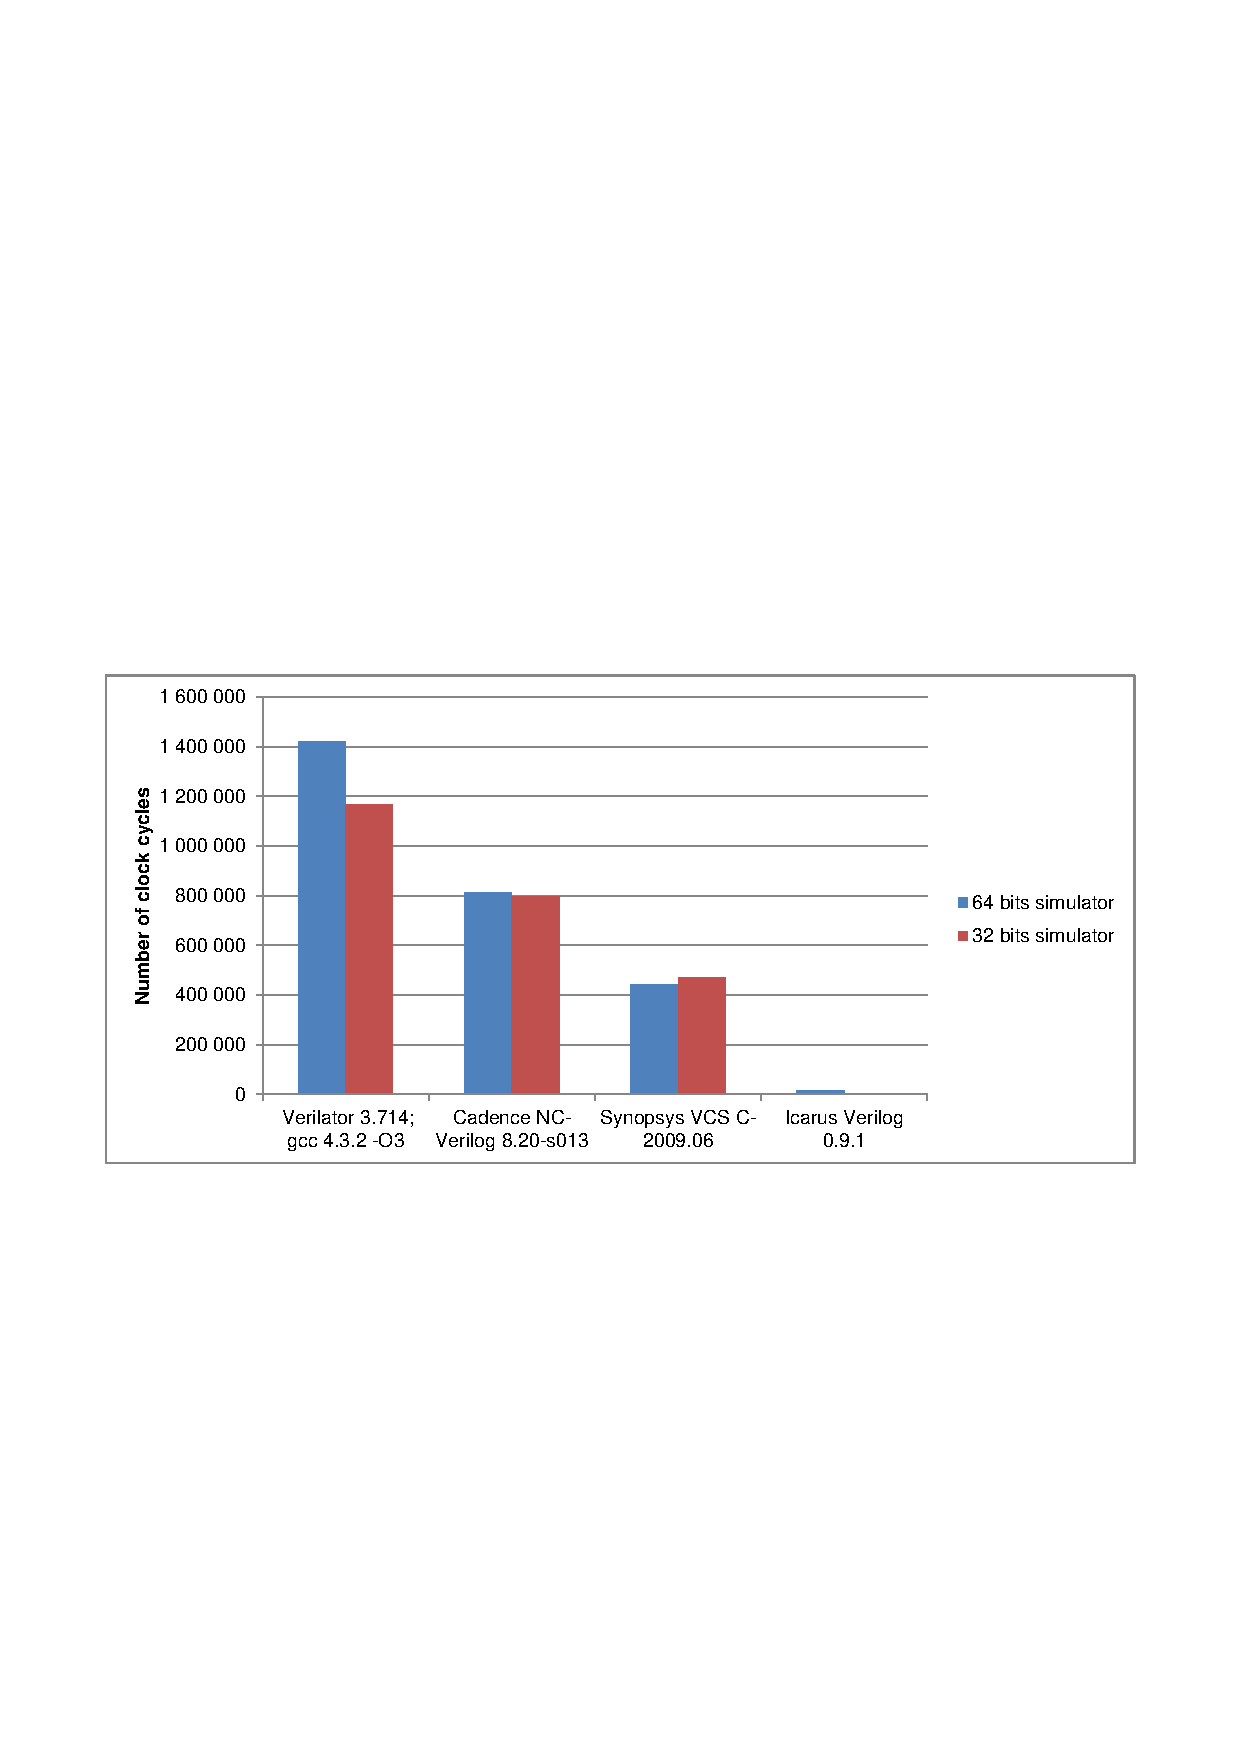
\includegraphics[trim=0 280 0 310 , clip, width=0.93\textwidth]{Figures/Performance.pdf}
	\caption{Benchmark results for different HDL simulators (higher means faster)~\cite{verilator:benchmarks}.}
	\label{fig:performance}
\end{figure}

The benchmark runs for the results shown in Figure~\ref{fig:performance} were
made in single-threaded mode. However, most commercial simulators (including the
ones analysed) support simulations in multi-threaded mode. This consists in
creating multiple threads for the different processes and distributing them
through multiple cores in a chip or even across multiple chips, that will be
executed in parallel. The threads are usually inter-dependent, so there should
be a synchronization process when transferring data between threads. This
process is time consuming, since different threads have different execution
times, requiring the faster threads to hold on until the slowest thread
finishes~\cite{tan:vhstas}.

Despite the concurrent nature of the Verilog statements, it isn't feasible to
parallelize the totality of the statements in a model, since the number of
statements is much greater than the amount of threads available, and also
because this would require a great amount of synchronization processes between
the different threads. Instead, the Verilog top-level code is divided in
multiple subsystems, with each one being simulated as a different thread.

The parallelization of HDL simulations is the solution found to achieve
considerable performance improvements in HDL simulators. This happens because
through the years the algorithms used in the simulators were optimized to such a
point where there were no further optimizations available, so the only viable
solution was to start using parallelization techniques.

%%  LocalWords:  parallelize
 % file "Thesis_Simulators.tex"
\cleardoublepage

\chapter{Simulating The RV32-Versat Architecture Using Event-Driven Simulators}
\label{chapter:sim_event}

In this chapter, the simulation environment for the RV32-Versat architecture
using commercially available event-driven simulators, more specifically the
Cadence NCsim and Synopsys VCS simulators, is detailed. As explained in the
previous chapter, event-driven simulators work by taking events sequentially,
propagating them through the circuit until the circuit reaches a steady
state~\cite{tan:vhstas,gunes:survey,palnitkar:verilog}. They produce accurate
simulation results with detailed timing information at the cost of the
simulation speed.

\section{Testbench}
\label{section:tb}

This type of simulators work with testbenches written in an \ac{HDL} such as
Verilog or VHDL. In Figure~\ref{fig:tb_verilog}, an example of a simple
testbench written in Verilog and used by NCSim and VCS is shown. This testbench
has RV32-Versat as the \ac{UUT} and uses a clock period of 10 ns, meaning that
the system is simulated at a frequency of 100 MHz. After 100 clock cycles with
the reset enabled ({\tt resetn=0}) the reset is disabled, and RV32-Versat starts
running. The data bus external ports are not used, since the memories are
initialized at compile time and no input hex file is loaded by the
testbench. The simulation finishes when the trap signal is activated (with {\tt
  resetn=0}), and if the flag VCD is passed when running the simulator a \ac{VCD}
file will be generated. The trap signal is activated when there is an invalid
memory access, which is useful for debug and for stopping the simulation, which
is caused by the user software that intentionally accesses the memory at a non
mapped location.

\lstset{language=verilog}
\begin{figure}[!htb]
	\begin{minipage}{\linewidth}
		\begin{spacing}{0.7}
			\begin{lstlisting}
			`timescale 1 ns / 1 ps
			
			module system_tb;
				reg clk = 1;
				always #5 clk = ~clk;
				
				reg resetn = 0;
				
				initial begin
					`ifdef VCD
						$dumpfile("system.vcd");
						$dumpvars();
					`endif
					repeat (100) @(posedge clk);
					resetn <= 1;
				end
				
				wire          led;
				wire          ser_tx;
				wire          trap;
				reg           databus_sel;
				reg           databus_rnw;
				reg [14:0]    databus_addr;
				reg [31:0]    databus_data_in;
				
				system uut (
					.clk             (clk        ),
					.resetn          (resetn     ),
					.led             (led        ),
					.databus_sel     (databus_sel),
					.databus_rnw     (databus_rnw),
					.databus_addr    (databus_addr),
					.databus_data_in (databus_data_in),
					.ser_tx          (ser_tx     ),
					.trap            (trap       )
				);
				
				initial begin
					databus_sel = 0;
					databus_rnw = 1;
					databus_addr = 0;
					databus_data_in = 0;
				end
				
				always @(posedge clk) begin
					if (resetn && trap) begin
						$finish;
					end
				end
			endmodule
			\end{lstlisting}
		\end{spacing}
	\end{minipage}
	\vspace*{-10mm}
	\caption{Example testbench in Verilog for RV32-Versat.}
	\label{fig:tb_verilog}
\end{figure}

\section{Verilog VPI}
\label{section:vpi}

The downside of using an HDL testbench with the event-driven simulators is their
limited support for software and hardware co-simulation. One way to overcome
this problem is to use the \ac{VPI}~\cite{vpi}, a C-programming interface for
Verilog that consists in a set of access and utility routines that are called
from standard C programming language functions. These routines interact with the
instantiated simulation objects contained in the Verilog design.

\lstset{language=C}
\begin{figure}[!htb]
	\begin{minipage}{\linewidth}
		\begin{spacing}{0.7}
			\begin{lstlisting}
			#include "vpi_user.h"
			
			void example() {
				vpi_printf("Example function\n");
				return;
			}
			\end{lstlisting}
		\end{spacing}
	\end{minipage}
	\vspace*{-10mm}
	\caption{Example C code for VPI.}
	\label{fig:vpi_c}
\end{figure}

To better explain how the~\ac{VPI} works there is a simple example of a C
function in Figure~\ref{fig:vpi_c}, called {\tt example.c} that prints text in
the terminal, using the {\tt printf} function from the \ac{VPI}. This function
now needs to be associated with a system task. For this, a special data
structure needs to be created, of the type {\tt vpi\_systf\_data}. The code for
the creation and registration of the system task can be seen in
Figure~\ref{fig:vpi_routine}. After this stage, the system task must be called
in the Verilog testbench of the circuit to simulate. This can be done either in
{\tt initial} blocks or in {\tt always} blocks. In Figure~\ref{fig:vpi_verilog}
an example using an {\tt initial} block is shown. The last thing to do is
linking the task with the simulator. This is usually made in the terminal when
calling the simulator.

\lstset{language=C}
\begin{figure}[!htb]
	\begin{minipage}{\linewidth}
		\begin{spacing}{0.7}
			\begin{lstlisting}
			#include "example.c"
			
			void hello_register()
			{
				s_vpi_systf_data tf_data; //data structure
			
				tf_data.type      = vpiSysTask; //does not return value
				tf_data.tfname    = "$hello"; //name of the task
				tf_data.calltf    = hello_calltf; //pointer for this routine
				tf_data.compiletf = hello_compiletf; //pointer for the compiled instance
																	  //of the task

				vpi_register_systf(&tf_data); //pointer to the structure
			}
			
			//Register the new task
			void (*vlog_startup_routines[ ]) () = {
				hello_register,
				0
			;}
			
			\end{lstlisting}
		\end{spacing}
	\end{minipage}
	\vspace*{-10mm}
	\caption{VPI task creation and registration.}
	\label{fig:vpi_routine}
\end{figure}

\lstset{language=Verilog}
\begin{figure}[!htb]
	\begin{minipage}{\linewidth}
		\begin{spacing}{0.7}
			\begin{lstlisting}
			module example ();
			
			initial begin
				$hello;
				#10 $finish;
			end
			   	  
			endmodule
			\end{lstlisting}
		\end{spacing}
	\end{minipage}
	\vspace*{-10mm}
	\caption{Verilog code to invoke the task.}
	\label{fig:vpi_verilog}
\end{figure}

As it can be seen, although it is possible to do software and hardware
co-simulation using Verilog testbenches, the process is not direct, making it a
disadvantage in simulation environments based on event-driven simulators. If the
low performance of this type of simulators is also taken into account (as it can
be seen in the benchmarks in Section~\ref{section:benchmark}), it can be
concluded that a simulation environment based on event-driven simulators does
not reach the objectives pretended: it is not fast, the simulators licences are
expensive and it does not provide a straightforward way of integrating hardware
and software co-simulation. Therefore, an alternative is necessary.  There is
another event-driven simulator (Icarus Verilog) that could solve the cost
problems, since it is free, but this simulator does not support the {\tt
  generate} loops used in the RV32-Versat Verilog code and has a very low
performance, as seen in Section~\ref{section:performance}.

 % file "Thesis_Event.tex"
\cleardoublepage

\chapter{Simulating The RV32-Versat Architecture Using The New Verilator Environment}
\label{chapter:sim_verilator}

In this chapter, the new simulation environment for the RV32-Versat architecture
using Verilator is detailed. The Verilator environment was designed to overcome
the disadvantages of typical simulation environments based on the more
traditional event-driven simulators, such as Cadence NCsim and the Synopsys VCS.
As detailed in the previous chapters these simulators are relatively slow,
require expensive licences and complicated the integration of hardware and
software, many times leading to the use of ad hoc solutions.

As explained in Chapter~\ref{chapter:simulators}, event-driven simulators
schedule and process events sequentially, and thus produce more accurate
simulation timing information at the cost of the simulation speed.

In contrast, Verilator is a cycle-accurate simulator and evaluates all logic
elements of the circuit for every clock cycle using binary (0/1) logic. This
produces less accurate results but the simulation is faster. This kind of
simulator does not evaluate any kind of timing in the circuit. However, it can
be used to quickly identify problems at an early stage or after a
change. Additionally, if the architecture is proven in other simulators or in
silicon, Verilator can be used to just capture behaviour modifications.


\section{Working Principle}
\label{section:working_principle}

The simulation environment created for RV32-Versat is based in a set of GNU
Makefiles~\cite{stallman:makefile}. In order to run the simulation environment
the user must go to the root of the RV32-Versat repository and type the command
{\tt make simulator\_name TEST=test\_name}, where the {\tt simulator\_name} is
the name of the desired simulator (Verilator) and {\tt test\_name} is the name
of the folder of the test (driving software program) that must be placed inside
of the folder {\tt tests/test\_name}. The test is compiled, the system memories
are initialized with the program code and data and the system is simulated, following the 
flow shown in Figure~\ref{fig:sim_flow}. This flow will be followed for any program that 
is created and simulated for this architecture.

\begin{figure}[!htb]
	\centering
	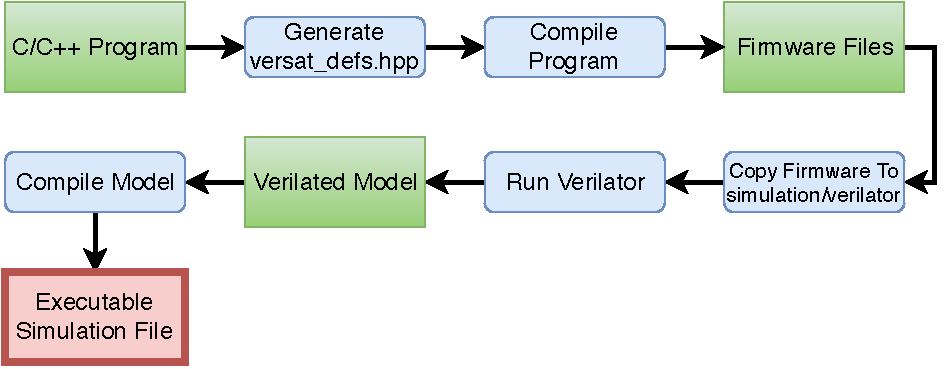
\includegraphics[width=0.95\textwidth]{Figures/Sim_flow.pdf}
	\caption{Simulation flow of the Verilator environment.}
	\label{fig:sim_flow}
\end{figure}

After the {\tt make} command is executed, the Makefile will call another
Makefile placed inside the folder {\tt simulation/verilator} that will then call
another Makefile placed inside the folder {\tt tests/test\_name}. This Makefile
generates the firmware hex files containing the RISC-V program and, if necessary, the 
data to be load into the Versat memories via the testbench, by generating the {\tt 
versat\_defs.hpp} file and compiling the program using the RISC-V toolchain.

The generated firmware files will then be copied into the {\tt simulation/verilator} 
folder where the respective Makefile was called. The next step is to call
Verilator to generate the Verilated model, a C++/System C model obtained from the
synthesizable Verilog files. This model is then linked to the testbench and compiled 
using GNU g++. The resulting executable simulation file will be run and perform 
the actual simulation.

An additional option was added that allows the simulation to be run in machines
that do not have the RISC-V toolchain~\cite{gnu:riscv} installed. This option
compiles the program via SSH in a remote machine where the toolchain is properly
installed. With this option, the user does not need to install the toolchain in
the computer where the simulator is installed, since installing the RISC-V toolchain can 
be a lengthy and complicated process. This option can be activated by adding the flag 
{\tt TOOLCHAIN=FALSE} in the make command.

\section{The Verilator Testbench}
\label{tb_verilator}

The Verilator testbench is considerably different from a typical HDL testbench,
mainly because it is written in C++, SystemC or a compination of both. The use
of these two languages instead of Verilog allows for much greater flexibility by
seamlessly emulating the software of a host system that stimulates the simulated
system. The testbench shown in Figure~\ref{fig:tb_cpp}, written in C++, works
essentially in the same way as the one shown in the previous chapter
(Figure~\ref{fig:tb_verilog}): it loads the hex files to the Versat memories via
the data bus and then runs the program. The simulation finishes when the trap
signal in the PicoRV32 processor is activated, together with an indication that
the program has finished. Optionally, the simulation can output an hex file with
the contents of the Versat memories using the data bus external ports.

\lstset{language=C++}
\begin{figure}[!htb]
	\begin{minipage}{\linewidth}
		\begin{spacing}{0.7}
			\begin{lstlisting}
			#include "Vsystem.h"
			#include "verilated.h"
			#include "verilated_vcd_c.h"
			
			vluint64_t main_time = 0; 
			double sc_time_stamp () {
			return main_time;
			}
			
			int main(int argc, char **argv, char **env)
			{
			Verilated::commandArgs(argc, argv);
			Verilated::traceEverOn(true);
			Vsystem* top = new Vsystem;
			VerilatedVcdC* tfp = new VerilatedVcdC;
			top->trace (tfp, 99);
			tfp->open ("waves.vcd");
			
			top->clk = 0;
			top->databus_sel = 0;
			top->databus_rnw = 1;
			top->databus_addr = 0;
			top->databus_data_in = 1;
			
			int t = 0;
			
			while (!Verilated::gotFinish()) {
			if (t > 200)
			top->resetn = 1;
			top->clk = !top->clk; //Toggle clock
			top->eval();          //Evaluate the model
			tfp->dump (t);        //Write to VCD file
			t += 5;               //Increment clock
			if (top->resetn && top->trap == 1)
			Verilated::gotFinish(true);
			}
			
			tfp->close(); //Close the VCD
			top->final(); //Finish the simulation
			delete top;
			exit(0);
			}
			\end{lstlisting}
		\end{spacing}
	\end{minipage}
	\vspace*{-10mm}
	\caption{Example testbench in C++ for RV32-Versat.}
	\label{fig:tb_cpp}
\end{figure}

The C++ header file created by Verilator from the Verilog model (the Verilated
model) must be included in the C++ testbench. After this, the {\tt
  sc\_time\_stamp} function is invoked, so that the simulator knows the current
time. The simulation setup is done in the {\tt main} function: the runtime
arguments are analysed ( {\tt commandArgs}), the computation of the traced
signals is enabled ( {\tt traceEverOn}), the module to be simulated is declared
( {\tt Vsystem*top}), along with the Verilated VCD model ( {\tt VerilatedVcdC*
  tfp}) and the number of hierarchy levels to be traced are defined ( {\tt
  top->trace (tfp, 99)}). As with the Verilog testbench example, in this example
the data bus external ports are switched off in order to keep the example
simple.

The clock of the circuit is toggled inside the while cycle. For each time that
this cycle executed, the clock signal will be negated, the simulation time will
be checked (to verify if the reset has been disabled), the circuit will be
evaluated ({\tt top->eval()}), the signals will be written to the VCD file ({\tt
  tfp->dump(t)}) and the clock signal time will incremented by 5 ns in each half
period, resulting in a frequency of 100 MHz.The testbench will be executed until
the ( {\tt Verilated::gotFinish}) condition is true. This will happen when the
trap signal is activated and the reset disabled (resetn=1), making the program
leave the while cycle. This will finish the simulation and exit the testbench.

Since the testbench is written in C++/SystemC, it is easy to do software and
hardware co-simulation, given that the host application can be directly embedded
in the testbench. This is a major improvement over other simulation environments
using Verilog testbenches. This is not the only advantage of this new
environment: the simulations using Verilator are considerably faster, as it can
be see in the benchmark presented in the Section~\ref{section:benchmark},
performed for the \ac{CNN} application presented in
Section~\ref{section:application}. Also, since Verilator is a completely free
open-source project, no licence fees are due. This advantages suit perfectly the 
objectives defined for the new simulation environment.
The major disadvantage of this new simulation environment is its lower
precision when compared with environments using event-driven simulators. This
happens because Verilator does not provide timing information, since it does not
take into account propagation times and because Verilator uses a 2-state model,
assuming that all the signals in a circuit have a value that can either be 0 or
1.  However, this disadvantage is many times irrelevant in the context of the
RV32-Versat architecture, since this architecture has already been extensively
tested in \ac{FPGA}s and with other simulators.

%%%%%%%%%%%%%%%%%%%%%%%%%%%%%%%%%%%%%%%%%%%%%%%%%%%%%%%%%%%%%%%%%%%%%%%%
 % file "Thesis_Verilator.tex"
\cleardoublepage

%%%%%%%%%%%%%%%%%%%%%%%%%%%%%%%%%%%%%%%%%%%%%%%%%%%%%%%%%%%%%%%%%%%%%%%%
%                                                                      %
%     File: Thesis_Results.tex                                         %
%     Tex Master: Thesis.tex                                           %
%                                                                      %
%     Author: Gonçalo Santos                                           %
%     Last modified : 20 Oct 2018                                      %
%                                                                      %
%%%%%%%%%%%%%%%%%%%%%%%%%%%%%%%%%%%%%%%%%%%%%%%%%%%%%%%%%%%%%%%%%%%%%%%%

\chapter{Results}
\label{chapter:results}

The aim of this work is to produce a workable {\bf C} language
compiler for the {\it Versat} architecture using the {\it picoVersat}
instruction set.
The success can be measured by the number of {\bf C} language
constructs that are working properly.
Consequently, testing is of primordial importance, as are the range
of tests used to exercise the compiler.

\section{Functionality}

The compiler, as far the tests were comprehensive,
supports all {\bf C} language integer constructs.
Limitations are listed below.

Since the processor instruction set is reduced, as are the
number of {\bf lcc} terminals to be implemented by the compiler,
the testing of each operation, on its own, is strait
forward.
Testing sequences of such operations may prove more
difficult to test, since different {\bf C} programs
can produce different selection matches.

\section{Testing}

In the test of a compiler, where a small change can affect the
generation of multiple instructions, a good set of
regressive tests is very important.
In order to automate the process, a {\tt test/} directory
was setup.
This directory includes a set of {\bf .c} test files and
the expected output {\bf .out}.

The {\tt Makefile} compiles, executes and compares the new
result with the previously stored result.
All differences in output are printed and can then be analyzed.

Since the output from {\bf iverilog} includes the number
of clocks spent, it is easy to compare whether the changes in the
compiler result in improvements, or in performance degradation.

Some tests are very simple and its output can be easily predicted.
To make testing even simpler, the return value of the {\tt main}
routine is printed, unless the {\sc NORET} environment variables
is defined. Upon return from the {\tt main} routine, the lowest
nibble is printed as an {\sc ASCII} starting at $0$.
This means that values between $10$ and $15$ are printed as
the {\sc ASCII} character at the respective offset, namely the
sequence: \verb|:|, \verb|;|, \verb|<|, \verb|=|, \verb|>|, \verb|?|.

More complex tests can be compiled with {\bf gcc} and executed
to access the expected output.
This, however, can not be performed if the examples include
{\tt asm} calls, since the code can only be executed by the
{\it Versat}, or by the {\bf iverilog} simulator, and not by the
native testbench processor.
%vdb.c

A set of $86$ regression tests is currently being used, ranging
from specific operator testing to complex recursive and iterative
examples. % And the number of tests keeps growing ...

\section{Limitations}\label{limitations}

The {\bf C} language imposes that {\tt sizeof(char)==1}
as does the {\bf lcc} compiler (see~\cite[p.79]{hanson95}).
This works fine as far as {\tt sizeof(char)} can be 32-bits.
However, additionally, the {\bf lcc} assumes through out
the code that $8$ is the number of {\em bit-per-byte}.
If it was a variable, one could set it to $32$.
As it is hardcoded, all address literals
will be truncated to 8-bits ({\tt 8}${}^{\wedge}${\tt ty->size}).
\begin{verbatim}
int *addr = (int*)0x123456;
\end{verbatim}
This can be avoided by setting an integer to the
required value and then assigning it to a pointer.
This works since integer literals are 32-bit wide
and the conversion to pointer, controlled by the
{\it back-end}, does not truncate the value.
\begin{verbatim}
int *addr, value = 0x123456;
addr = (int*)value;
\end{verbatim}
Nevertheless, defining literal pointer is never
a good predictive in virtual memory machines.
In {\it Versat} it is useful to map variables
to specific addresses.

Due to the same reason, a warning message is issued
({\tt shifting an `int' by 12 bits is undefined})
but the code is correctly generated.

% #define LONG_MIN -2147483648
% warning: unsigned operand of unary -
% but 0x80000000 or bellow is OK!
% #  define LONG_MAX	2147483647
% #  define LONG_MIN	(-LONG_MAX - 1L)

In the initial version of {\it picoVersat}, all global
data must be added by {\tt MEM\_BASE=512}.
Since this is performed when addresses are fetched,
static assignments store the unadded value.
Therefore, all accesses must be added by $512$.
Must add {\tt 512} to global pointers in {\tt picoversat-0.0}
\begin{verbatim}
int mem[10], *base = mem;
int main() { base[6+512] = 9; return return mem[6]; }
\end{verbatim}
This can be avoided if assignment is performed during
execution (not at compile time), even if the variable
is global.
\begin{verbatim}
int mem[10];
int main() { int *base = mem; base[6] = 9; return return mem[6]; }
\end{verbatim}

Signed multiplication, division and modulus ({\tt \_mul},
{\tt \_div} and {\tt \_mod}) do not generate carry since
the flags register of {\it picoVersat} is read-only.

The {\bf C} programming languages relies on separate
compilation, where several files are independently
compiled and then linked together.
However, there is no linker in the {\it Versat} system
and the assembler {\bf va} does not support multiple
files.
The solution is to perform linking with {\bf cpp} %%%
include directives.
While in normal {\bf C} the {\tt .c} should be
included, rather compiled, the inclusion of {\bf .h}
as well as {\bf .c} accomplishes the desired result.
Since there is no linking, only multiple inclusion
of files must be avoided.

The {\it Versat} architecture is meant to be used offline
and no form of argument passing to the {\tt main} routine
is available.
Consequently, the stack is initialized at the top.
Therefor, even if the program declares arguments to
the {\tt main} routine ({\tt argc, argv, envp}) they should
never be accessed.
Also, since the system has no memory management unit,
all illegal accesses are silently ignored by the system.
Highly recursive routines that exhaust the stack will have
unpredictable behaviors, since they will begin to overwrite
the top of the code.
Even if it is not the compilers responsibility, it something
that the programmer should be aware, especially when
transitioning from a virtual managed memory system.

Finally, the compiler does not support floating point
data types, since every operation must be supported
by library routines.
This is the case for many android devices, namely
smartphones.
However, the {\it Versat} purpose is to perform
integer arithmetic operations fast and is not aimed at
scientific programming.
The error message {\tt compiler error in \_label--Bad terminal}
is issued by the compiler when it cannot handle a given operation,
namely floating point operations.

\section{Register assignment}

Register assignment in compiler design considers two types of registers:
global registers that hold variable values and scratch registers that hold
temporary values.
The {\bf lcc} compiler defines these registers by setting a mask for each
type of register.
It is up to each {\it back-end} to define the mask values according to processor
capabilities.
For instance, the {\bf sparc} processor defines $4$ sets of $8$ registers:
global, temporary, input and output; where the later two sets replace
the stack for argument passing.
In {\bf i386} all $7$ registers are temporary, while {\bf mips} uses half
for each purpose ($16+16$).

Since the {\it picoVersat} has no specific register assignment, a study
was carried out in order to assess the best balance between global and
scratch registers.
Registers {\tt R0} and {\tt R13} to {\tt R15} are used to communicate with {\it Versat}
and are invisible to the compiler.
The stack is controlled by a {\it stack pointer} ({\tt R12}) and a {\it frame pointer}
({\tt R11}).
The remaining registers ({\tt R1} to {\tt R10}) compose a mask {\tt 7FE}, where
the lowest bit ({\tt R0}) is omitted for register assignment, and the highest
used bit {\tt 400} is {\tt R10}.
The register {\tt R1} is used to return function values and all arguments are
passed on the stack.
At least two registers must be used as scratch for binary operations
temporaries.
The compiler allows the definition of a {\tt tmask} for temporaries and a
{\tt vmask} for variables.

Initially, in run $1$, the experiment uses all registers for temporaries.
Each run adds a variable register at the expense of a temporary, until only
two temporaries remain (run $9$).
Three examples where used: {\tt assign}, {\tt repeating locals} and
{\tt bubble sort}.
The first two represent opposite extremes of register usage, while the last is
a more balanced and realistic example.

The first example uses the {\bf C} language right associative {\it assign} operator
where each new assignment to the variable {\tt a} requires a new temporary register.
%(see Figure~\ref{fig:assign}).

%\begin{figure}
\begin{verbatim}
int f() { return 1; }
int main()
{
  int a;

  a = f() + (a =
      f() + (a =
      f() + (a =
      f() + (a =
      f() + (a =
      f() + (a =
      f() + (a =
      f() + (a =
      f() + (a =
      f() + (a =
      f() + (a =
      f() + (a =
      f() + (a = 1
                  )))))))))))));
  return a;
}
\end{verbatim}
%\caption{}
%\end{figure}

The register usage shows that each assign uses a register $4$ times at
the expense of the return register {\tt R1}.
The best solution, represented by the lowest clock count,
is to use only two temporaries, since more variables imply more stack ({\tt R12}),
saves and restores between each call to the function {\bf f}.

%\begin{table}
\begin{center}
{\small
\begin{tabular}{r|r|r|r|r|r|r|r|r|r|r|r|r|r|r|r|r}
run&vars&vmask&tmask&R1&R2&R3&R4&R5&R6&R7&R8&R9&R10&R11&R12&clks\\\hline
1&0&000&7FE&21&4&4&4&4&4&4&4&6&44&27&82&677\\
2&1&400&3FE&23&4&4&4&4&4&4&6&42&17&14&82&638\\
3&2&600&1FE&25&4&4&4&4&4&6&42&0&17&16&77&633\\
4&3&700&0FE&27&4&4&4&4&6&42&0&0&17&18&72&628\\
5&4&780&07E&29&4&4&4&6&42&0&0&0&17&20&67&623\\
6&5&7C0&03E&31&4&4&6&42&0&0&0&0&17&22&62&618\\
7&6&7E0&01E&33&4&6&42&0&0&0&0&0&17&24&57&613\\
8&7&7F0&00E&35&6&42&0&0&0&0&0&0&17&26&52&608\\
9&8&7F8&006&39&42&0&0&0&0&0&0&0&17&28&47&603\\
\end{tabular}
}
\end{center}
%\caption{}
%\end{table}
\vspace*{5mm}

The second example uses lots of repeating local variables so that each one is assigned
a register, for its uses from the first to last line, if one is available.
%(see Figure~\ref{fig:locals}).

%\begin{figure}
\begin{verbatim}
int func(int a, int b, int c, int d, int e, int f, int g, int h, int i, int j, int k) {
    a = a + b - c - d - e + f - g + h + i + j + k;
    b = a - b + c + d - e - f + g - h + i - j - k;
    c = a + b - c - d + e + f + g - h + i + j - k;
    d = a - b - c + d - e + f - g + h - i - j - k;
    e = a + b + c - d - e - f - g + h - i + j - k;
    f = a - b - c + d - e + f + g - h - i - j + k;
    g = a + b - c - d + e + f + g - h + i + j - k;
    h = a - b + c + d - e - f - g + h + i - j - k;
    i = a + b - c - d - e + f + g + h + i + j - k;
    j = a - b - c + d - e + f + g - h - i - j - k;
    k = a + b + c - d + e - f - g - h - i + j + k;
    return a + b + c + d + e + f - g + h - i + j - k;
}

int main() {
    return func(10, 9, 8, 7, 6, 5, 4, 3, 2, 1, 0);
}
\end{verbatim}
%\caption{}
%\end{figure}

As expected, the best solution is to use highest of temporaries in order
to reduce frame pointer ({\tt R11}) accesses to stack saved values.

%\begin{table}
\begin{center}
{\small
\begin{tabular}{r|r|r|r|r|r|r|r|r|r|r|r|r|r|r|r|r}
run&vars&vmask&tmask&R1&R2&R3&R4&R5&R6&R7&R8&R9&R10&R11&R12&clks\\\hline
1&0&000&7FE&45&27&12&13&48&46&40&45&54&62&68&56&956\\
2&1&400&3FE&53&31&13&54&46&40&47&54&62&0&78&51&1001\\
3&2&600&1FE&61&35&52&46&48&49&56&62&0&0&89&46&1051\\
4&3&700&0FE&89&39&59&63&51&56&62&0&0&0&101&41&1106\\
5&4&780&07E&109&43&75&49&74&79&0&0&0&0&113&36&1161\\
6&5&7C0&03E&146&45&84&58&105&0&0&0&0&0&124&31&1211\\
7&6&7E0&01E&156&88&112&94&0&0&0&0&0&0&138&26&1278\\
8&7&7F0&00E&171&117&176&0&0&0&0&0&0&0&154&21&1356\\
9&8&7F8&006&231&249&0&0&0&0&0&0&0&0&172&16&1447\\
\end{tabular}
}
\end{center}
%\caption{}
%\end{table}
\vspace*{5mm}

The last example, the {\it bubble sort}, uses a mixture temporaries and variable
reuses. %(see Figure~\ref{fig:bubble}).

%\begin{figure}
\begin{verbatim}
#include "printi.h"

int bubble(int list[], int n) {
    int c, d, t, swap, cnt = 0;

    for (c = 0; c < n - 1; c++) {
        for (swap = 0, d = n - 1; d > c; d--)
            if (list[d - 1] > list[d]) {    /* Swapping */
                swap++;
                t = list[d];
                list[d] = list[d - 1];
                list[d - 1] = t;
            }
        if (!swap)
            break;
        cnt++;
    }
    return cnt;
}

int v[] = { 7, 4, 9, 6, 2, 1, 3, 5, 8, 0 };

int main() {
    int i, size = sizeof(v) / sizeof(v[0]), cnt = bubble(v, size);
    for (i = 0; i < size; i++) {
        putchar(v[i] + '0');
        putchar(' ');
    }
    printi(cnt, 10);
    putchar('\n');
    return 0;
}
\end{verbatim}
%\caption{}
%\end{figure}

This example exploits the tradeoff between global and temporary register
usage.
In the first runs the compiler is unable to use all temporaries.
In the last runs some variable registers are left unassigned and the number
of required execution clocks rises again.

%\begin{table}
\begin{center}
{\small
\begin{tabular}{r|r|r|r|r|r|r|r|r|r|r|r|r|r|r|r|r}
run&vars&vmask&tmask&R1&R2&R3&R4&R5&R6&R7&R8&R9&R10&R11&R12&clks\\\hline
1&0&000&7FE&2&0&0&0&0&4&5&15&30&45&31&36&9855\\
2&1&400&3FE&2&0&0&0&0&4&7&29&41&11&24&36&8193\\
3&2&600&1FE&2&0&0&0&4&5&27&37&7&11&19&41&7714\\
4&3&700&0FE&2&0&0&0&5&25&37&4&7&11&17&41&7399\\
5&4&780&07E&2&0&0&5&19&37&6&4&7&11&13&46&7022\\
6&5&7C0&03E&2&0&5&19&33&6&6&4&7&11&9&49&6949\\
7&6&7E0&01E&2&5&19&33&0&6&6&4&7&11&9&49&6949\\
8&7&7F0&00E&5&19&33&0&0&6&6&4&7&11&9&44&6921\\
9&8&7F8&006&21&28&0&0&0&6&6&4&7&11&13&41&7492\\
\end{tabular}
}
\end{center}
%\caption{}
%\end{table}
\vspace*{5mm}

Based on experience with the examples above, a balanced approach should work best
in most cases.
Therefor, the first five registers, {\tt R1} to {\tt R5}, are used as temporaries
({\tt tmask=0x003E}) and the remaining five, {\tt R6} to {\tt R10}, are used as
variables ({\tt vmask=0x07C0}).

\section{Efficiency considerations}

Calls are very expensive operations for any processor.
{\it Intel Inc.} has made a significant effort over the year to address this
problem.
In the last years, its high end processors provide faster {\it calls} than
{\it jumps} at the expense of higher transistor count. %ref!
In a processor like {\it picoVersat}, the problem is magnified since
no stack specific registers or opcodes are available.

A function call in the {\bf C} programming language requires:
\begin{enumerate} \itemsep0em 
\item {\bf argument passing} by pushing values to the stack;
\item {\bf calling} the desired routine;
\item {\bf saving used registers} before the routine destroys its values;
\item {\bf frame pointer} saving to access arguments and locals;
\item {\bf allocate space} for local variables;
\item actually performing the routine operations;
\item {\bf restoring frame pointer} of the previous routine;
\item {\bf restoring used registers} previous values;
\item {\bf returning} to the calling routine;
\item {\bf removing arguments} from stack.
\end{enumerate}
The present compiler detects when a routine accesses no arguments or locals
and does not emit frame pointer code. So, if a routine only uses global
variables, the call becomes a bit more efficient.
Some of the tests used become upto 5\% faster by removing the frame
pointer in routines where it not needed.

As any routine can be called many times, even recursively, the compiler
must save, at the beginning, and restore, at the end,
all the registers the routine uses.
This means that, at the start of the program, the {\tt main} routine will spill
all registers it will use, although they have no defined value.
Such procedure is required since the routine may be recursively called.
However, in most cases, the {\tt main} routine is only invoked once, at
the start of the program.
The {\sc NOSAV} environment variable can be set if the {\tt main}
routine is not used recursively and no registers will saved by the compiler.
This special hack can be dangerous to use, but it makes {\tt main} based
programs more efficient.

The {\it picoVersat} controls {\it Versat} by setting specific values to
predefined memory positions.
The use of a routine to perform such a task is a very
expensive way to change memory positions, either through {\tt asm}
directives or standard {\bf C} code, as the tests {\tt set.c} and
{\tt setvar.c} show, respectively.
Memory values can be efficiently changed by assigning to a pointer
{\tt *addr=val} (see Limitations, above).

During this work, the {\it picoVersat} evolved. The use of a single
memory, for program code and data, removed the need for a {\tt addi MEM\_BASE}
instruction for each variable load and store, resulting in a 5\% improvement
over all the regression test in use, at the time. % 17022/16213 pico-0

Finally, the compiler some times generates a register read after the
same register was written by another instruction selection.
At least, the read can be suppressed, but {\bf lcc} provides no
peephole optimizer for final code cleanup.

\section{Compiler instalation}

The compiler itself, {\bf lcc}, can be invoqued directly with the
{\tt -target=versat} option, as long as the input file has already
been preprocessed ({\bf cpp}).
The compiler output is a {\it picoVersat} assembly, that can then
fed to the {\it versat} assembler ({\bf va}).

However, the complete compilation process, from {\bf C} language
source file to {\bf iverilog} simulation executable, can be
integrated as in a standard high-level compiler.

Section~\ref{app:integ} describes the requirements for such an integration.
The compiler {\tt Makefile}s, in the main and {\tt versat/} directories,
can be used to provide the instalation of all required files
for a complete development environment.
By default, without any changes to the {\tt Makefile}s, the
compiler development environment is placed under the
{\tt /usr/local/versat} directory.

The default directories for the compiler installation
({\tt make install}) are predefined as
{\tt /usr/local/versat/lcc} for the compiler files
({\tt lcc}, {\tt cpp}, {\tt rcc}, {\tt va}, and
{\tt xdict.json}), and can be redefined at compile
time or using the {\sc LCCDIR} environment variable
at runtime. The {\it picoVersat} {\tt rtl/} files
({\tt include/}, {\tt src/}, and {\tt testbench/})
should be copied to {\tt /usr/local/versat/pico}
(defined at compile time).
Also the {\bf iverilog} compiler is defined at
compile time as residing in {\tt /usr/local/bin/}.

The structure of the installed files,
in the current version is:
\begin{Verbatim}[baselinestretch=1.0]
/usr/local/versat/lcc/lcc
/usr/local/versat/lcc/cpp
/usr/local/versat/lcc/rcc
/usr/local/versat/lcc/va
/usr/local/versat/lcc/xdict.json
/usr/local/versat/lcc/include/strlen.h
/usr/local/versat/lcc/include/umod.h
/usr/local/versat/lcc/include/errno.h
/usr/local/versat/lcc/include/malloc.h
/usr/local/versat/lcc/include/umul.h
/usr/local/versat/lcc/include/itoa.h
/usr/local/versat/lcc/include/Makefile
/usr/local/versat/lcc/include/stdarg.h
/usr/local/versat/lcc/include/mem_ends.h
/usr/local/versat/lcc/include/xdict.h
/usr/local/versat/lcc/include/atoi.h
/usr/local/versat/lcc/include/puts.h
/usr/local/versat/lcc/include/dma.h
/usr/local/versat/lcc/include/versat.h
/usr/local/versat/lcc/include/ends.h
/usr/local/versat/lcc/include/mul.h
/usr/local/versat/lcc/include/xdictinc
/usr/local/versat/lcc/include/div.h
/usr/local/versat/lcc/include/ends.cbc
/usr/local/versat/lcc/include/udiv.h
/usr/local/versat/lcc/include/printf.h
/usr/local/versat/lcc/include/mod.h
/usr/local/versat/lcc/include/alloca.h
/usr/local/versat/lcc/include/printi.h
/usr/local/versat/lcc/include/gnuc.h
/usr/local/versat/lcc/include/putchar.h
/usr/local/versat/lcc/include/assign.h
/usr/local/versat/pico/testbench/sim_xtop.cpp
/usr/local/versat/pico/testbench/xtop_tb.v
/usr/local/versat/pico/include/xdefs.vh
/usr/local/versat/pico/src/xaddr_decoder.v
/usr/local/versat/pico/src/xctrl.v
/usr/local/versat/pico/src/xram.v
/usr/local/versat/pico/src/xregf.v
/usr/local/versat/pico/src/xcprint.v
/usr/local/versat/pico/src/xtop.v
\end{Verbatim}

After adding the {\tt /usr/local/versat/lcc} directory to
the {\sc PATH} environment variable, an executable example
can be produced with the command:\\
{\tt lcc example.c -o example}

The example can then be run with:\\
{\tt ./example}

Please note that the {\it versat} memory dump {\tt .hex}
file is stored in the {\tt /tmp} directory.

\cleardoublepage
 % file "Thesis_Results.tex"
\cleardoublepage

%\input{Thesis_new_file} % add new .tex files for new chapters
% \cleardoublepage

%\input{Thesis_new_file} % add new .tex files for new chapters
% \cleardoublepage

%\input{Thesis_new_file} % add new .tex files for new chapters
% \cleardoublepage

%%%%%%%%%%%%%%%%%%%%%%%%%%%%%%%%%%%%%%%%%%%%%%%%%%%%%%%%%%%%%%%%%%%%%%%%
%                                                                      %
%     File: Thesis_Conclusions.tex                                     %
%     Tex Master: Thesis.tex                                           %
%                                                                      %
%     Author: Carlos A. Rodrigues                                      %
%     Last modified : 21 Jan 2011                                      %
%                                                                      %
%%%%%%%%%%%%%%%%%%%%%%%%%%%%%%%%%%%%%%%%%%%%%%%%%%%%%%%%%%%%%%%%%%%%%%%%

\chapter{Conclusão}
\label{chapter:conclusao}

Insert your chapter material here...


% ----------------------------------------------------------------------
\section{Achievements}
\label{section:achievements}

The major achievements of the present work...


% ----------------------------------------------------------------------
\section{Trabalho Futuro}
\label{section:futuro}

dese


\cleardoublepage

 % file "Thesis_Conclusions.tex"
\cleardoublepage

% ----------------------------------------------------------------------
%  Bibliography
% ----------------------------------------------------------------------

% Add entry in the table of contents as chapter
\phantomsection
\addcontentsline{toc}{chapter}{\bibname}

% Include all references in .bib file, even non-cited ones...
%\nocite{*} % this should be used carefully because it is not correct!

% Produces the bibliography section when processed by BibTeX
%
% Bibliography style
% > entries ordered alphabetically
%\bibliographystyle{plain}
% > unsorted with entries appearing in the order in which the citations appear.
%\bibliographystyle{unsrt}
% > entries ordered alphabetically, with first names and names of journals and months abbreviated
%\bibliographystyle{abbrv}
% > entries ordered alphabetically, with reference markers based on authors' initials and publication year
%\bibliographystyle{alpha}
%
% Replacement bibliography styles provided by 'natbib' package
% (plainnat.bst, abbrvnat.bst, unsrtnat.bst )
% > entries ordered alphabetically
%\bibliographystyle{plainnat}
% > unsorted with entries appearing in the order in which the citations appear.
%\bibliographystyle{unsrtnat}
% > entries ordered alphabetically, with first names and names of journals and months abbreviated
%\bibliographystyle{abbrvnat} % <<<<< SELECT IF USING REFERENCES BY AUTHOR/YEAR
% > entries ordered alphabetically, with reference markers based on authors' initials and publication year
%\bibliographystyle{alpha}
%
% Custom bibliography style adapted from 'natbib' package
%   (based on http://tex.stackexchange.com/questions/5053/is-it-possible-to-get-unsrt-abbrv-bibliography)
%   (unsrtnat.bst + abbrvnat.bst -> abbrvunsrtnat.bst)
%   (original files copied from:
%   http://tug.ctan.org/macros/latex/contrib/natbib/abbrvnat.bst
%   http://tug.ctan.org/macros/latex/contrib/natbib/unsrtnat.bst
% > unsorted with entries appearing in the order in which the citations appear, with first names and names of journals and months abbreviated.
\bibliographystyle{abbrvunsrtnat} % <<<<< SELECT IF USING REFERENCES BY NUMBER (CITATION ORDER)

% External bibliography database file in the BibTeX format
\bibliography{Thesis_bib_DB} % file "Thesis_bib_DB.bib"

%\cleardoublepage

% ----------------------------------------------------------------------
%  Appendix (optional)
%
%  CAUTION: 1) the main document (up to the conclusions) shall not exceed 80 pages
%           2) the document shall not exceed a total of 100 pages (per IST regulations)
% ----------------------------------------------------------------------
\appendix

% add page number prefix according to apendix chapter (optional)
%\renewcommand{\thepage}{\thechapter.\arabic{page}}

% re-set arabic numbering (A.1,A.2,...) (optional, use only if chapter prefix is added)
%\setcounter{page}{1}

%%%%%%%%%%%%%%%%%%%%%%%%%%%%%%%%%%%%%%%%%%%%%%%%%%%%%%%%%%%%%%%%%%%%%%%%%
%                                                                      %
%     File: Thesis_Appendix_A.tex                                      %
%     Tex Master: Thesis.tex                                           %
%                                                                      %
%     Author: Andre C. Marta                                           %
%     Last modified :  2 Jul 2015                                      %
%                                                                      %
%%%%%%%%%%%%%%%%%%%%%%%%%%%%%%%%%%%%%%%%%%%%%%%%%%%%%%%%%%%%%%%%%%%%%%%%

\chapter{Vector calculus}
\label{chapter:appendixVectors}

In case an appendix if deemed necessary, the document cannot exceed a total of 100 pages...

Some definitions and vector identities are listed in the section below.

% ----------------------------------------------------------------------
\section{Vector identities}
\label{section:vectorIdentities}

\begin{equation}
	\nabla \times \left( \nabla \phi \right) = 0
	\label{eq:cross_nnp}
\end{equation}

\begin{equation}
	\nabla \cdot \left( \nabla \times {\bf u} \right) = 0
	\label{eq:dotCross_nnu}
\end{equation}

 % file "Thesis_Appendix_A.tex"
%\cleardoublepage

% re-set arabic numbering (B.1,B.2,...) (optional, use only if chapter prefix is added)
%\setcounter{page}{1}

%%%%%%%%%%%%%%%%%%%%%%%%%%%%%%%%%%%%%%%%%%%%%%%%%%%%%%%%%%%%%%%%%%%%%%%%%
%                                                                      %
%     File: Thesis_Appendix_B.tex                                      %
%     Tex Master: Thesis.tex                                           %
%                                                                      %
%     Author: Andre C. Marta                                           %
%     Last modified :  2 Jul 2015                                      %
%                                                                      %
%%%%%%%%%%%%%%%%%%%%%%%%%%%%%%%%%%%%%%%%%%%%%%%%%%%%%%%%%%%%%%%%%%%%%%%%

\chapter{Technical Datasheets}
\label{chapter:appendixDatasheets}

It is possible to add PDF files to the document, such as technical sheets of some equipment used in the work.

% ----------------------------------------------------------------------
\section{Some Datasheet}
\label{section:datasheet}

% See more options to include PDF files in
% http://mirror.unl.edu/ctan/macros/latex/contrib/pdfpages/pdfpages.pdf
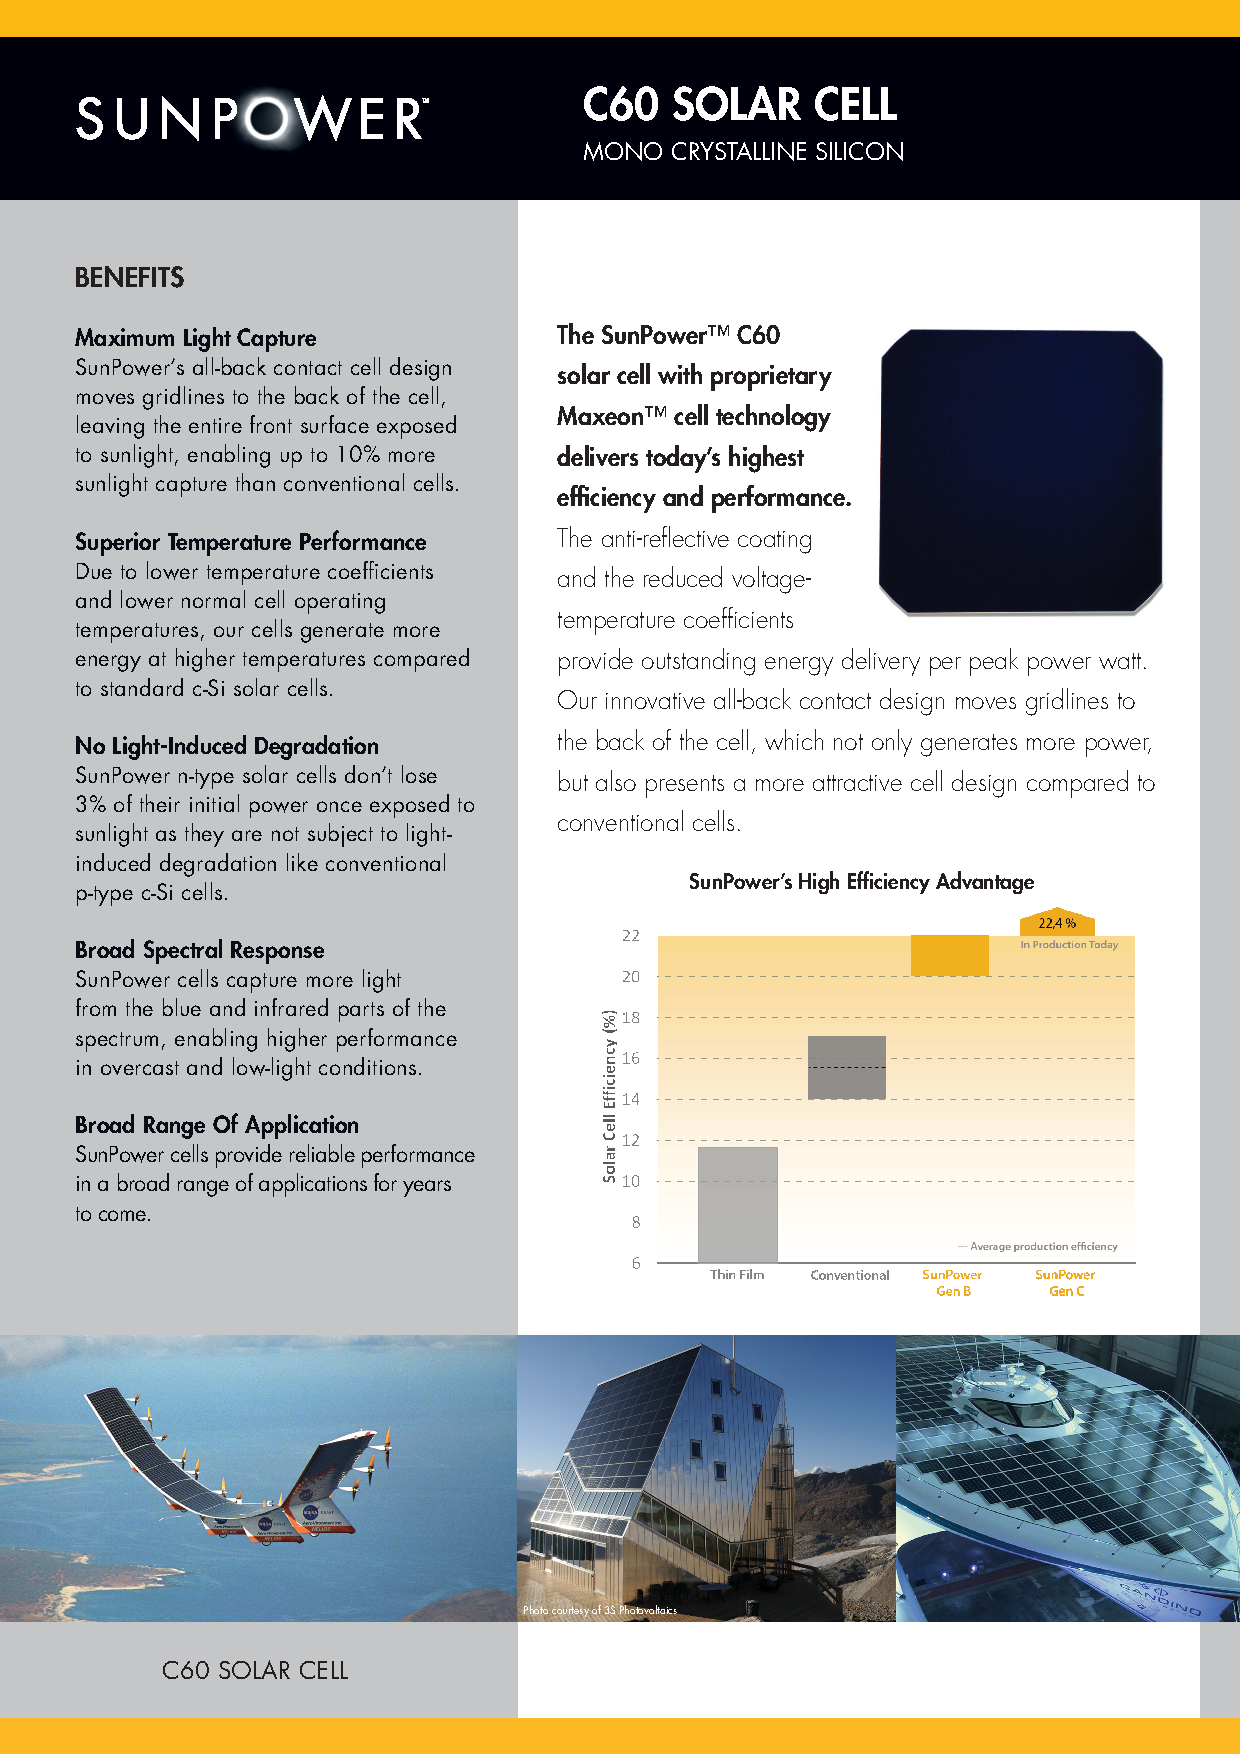
\includepdf[pages={1-2},nup=1x2,landscape=true]{Figures/SolarCell_Sunpower_C60.pdf}

 % file "Thesis_Appendix_B.tex"
%\cleardoublepage

% ----------------------------------------------------------------------
\end{document}
% ----------------------------------------------------------------------

